\section{Introduction}

Integrity is doing the right thing even when no one is watching. - C.S. Lewis. Computational integrity (CI) refers to the assurance that a computation is well done executed and the results of that execution are accurate, reliable, and trustworthy. This document describes the assembly language created by Polygon, designed specifically with Ethereum Virtual Machine (EVM) features to represent blockchain transactional-based computations that could be executed with probable CI.


Ethereum is a decentralized, general-purpose blockchain computer where programs are represented as smart contracts and state transitions are triggered by users through the execution of transactions. One of the key components of Ethereum is the EVM. The EVM is a runtime environment that executes smart contracts on the Ethereum network. It provides a secure and isolated environment for executing code, and it ensures that the code is executed in a predictable and deterministic manner. 

When executing a transaction on the Ethereum network, a fee must be paid. The fee is proportional to the complexity of the computation and the demand on the network. The increasing demand for the Ethereum network, combined with its limited capacity, has caused the fees to rise to the point where they may impact the practical usability of the network. To address this issue, several layer 2 (L2) solutions have emerged in the market to improve the usability of Ethereum.

Polygon's zkEVM is a layer 2 network that implements a special instance of the Ethereum Virtual Machine (EVM). Although the network has a different architecture and state from Ethereum layer 1 (L1), communication with the Polygon zkEVM is done through a JSON-RPC interface that is fully compatible with Ethereum RPC, allowing all Ethereum-compatible applications and tools to be natively compatible with Polygon zkEVM. However, it's important to note that this is a separate instance with a distinct state from Ethereum L1, and as such, balances in accounts may not be the same and L1 smart contracts cannot be directly accessed through L2 transactions. Nevertheless, a bridge and cross-chain messaging mechanism enables the exchange of data between both networks (refer to the technical documents regarding the zkEVM bridge).

\subsection{EVM interpreter}

EVM interpreter is a software component that can process and execute Ethereum transactions. 

Ethereum smart contracts can be written in various programming languages, such as Solidity, Vyper, Fe, or Yul, but are ultimately compiled into a sequence of EVM opcodes, expressed as bytecodes, that can be interpreted by the EVM interpreter. Ethereum opcodes are the low-level instruction set for EVM and represent the basic operations that EVM can perform during the execution of a smart contract triggered by a transaction.

The list of Ethereum op codes includes over 200 different operations , ranging from general arithmetic and logical operations to more advanced and blockchain eviroment specific operations like calls to other contracts, contract creation, and storage management. Some of the most commonly used op codes include:

\begin{itemize}
\item \textbf{ADD, SUB, MUL, DIV:} Basic arithmetic operations.
\item \textbf{CALL, DELEGATECALL, CALLCODE:} Calling other contracts.
\item \textbf{PUSH, POP:} Stack management operations.
\item \textbf{JUMP, JUMPI:} Conditional jumps for making decisions.
\item \textbf{SLOAD, SSTORE:} Storage management operations.
\item \textbf{MLOAD, MSTORE:} Memory management operations.
\end{itemize}

\subsection{zkASM and the ROM}
The zero-knowledge Assembly (zkASM) is an assembly language designed by Polygon to describe computations that can be executed by a "special" virtual machine. This virtual machine has the ability to not only compute an output from a computation description and a set of inputs, but also generate a succinct cryptographic CI proof of a fixed length. This proof can be verified using a fixed and, more importantly, a low amount of energy and time. To achieve this “special” behavior, this virtual machine relies on Zero Knowledge technology. 

Therefore, for any computation described in zkASM and executed with this "special" virtual machine its CI can be verified using fewer computational resources than were required for the original computation. The trick is that the proof verification algorithm can be implemented using a Ethereum smart contracts language and deployed on Ethereum L1, so for any computation expressed in zkASM its CI can be efficiently verified on Ethereum L1 using a fixed and low amount of gas, thereby inheriting Ethereum L1 security while avoiding network overhead. 

In Ethereum L1, transactions are grouped into blocks. Each block contains an ordered sequence of transactions that are executed in a deterministic manner over Ethereum state, resulting in a new version of the Ethereum L1 state. Unlike Ethereum L1, in Polygon's zkEVM, the data structure that contains an ordered set of transactions that represents a state transition, is called a batch.

The ROM is a zkASAM program that is an EVM interpreter for Polygon zkEVM's batches architecture, all EVM opcodes are implemented on it aswell the batch interpretation and transaction execution logic in such a way that by the use of the ROM, our "special" virtual machine, given an Polygon's zkEVM L2 State and a batch of transactions, can execute those transactions, compute the resulting L2 State and generate a CI proof of the state transition. In order to verify the CI proofs, and provide data availability to the batches data, a sophisticated protocol has been designed and deployed on Ethereum L1 (refer to the technical documents regarding the zkEVM state management). The advantage of this design is that it enables the creation of a highly efficient Ethereum network (Polygon zkEVM) on top of Ethereum L1, inheriting its security, moreover most of the Ethereum ecosistem will be natively compatible with this new network. ROM stands for Read-Only Memory, due to its analogy with computer memories. Indeed the system can be viewed as a silicon processor capable of interpreting a set of instructions and a ROM memory containing a firmware (a piece of low-level software that is infrequently subjected to changes) written with that set of instructions which implements a special EVM interpreter for Polygon zkEVM L2 architecture. To operate, the processor executes the ROM's program which takes as inputs a batch of L2 transactions to be executed and the previous L2 State, and produces a new state and a CI proof as output. The system composed of the zk "special" virtual machine and the ROM is called the zkEVM batch prover.

Figure 1 shows a high level overview of the zkEVM batch prover.

\begin{figure}[H]
\centering
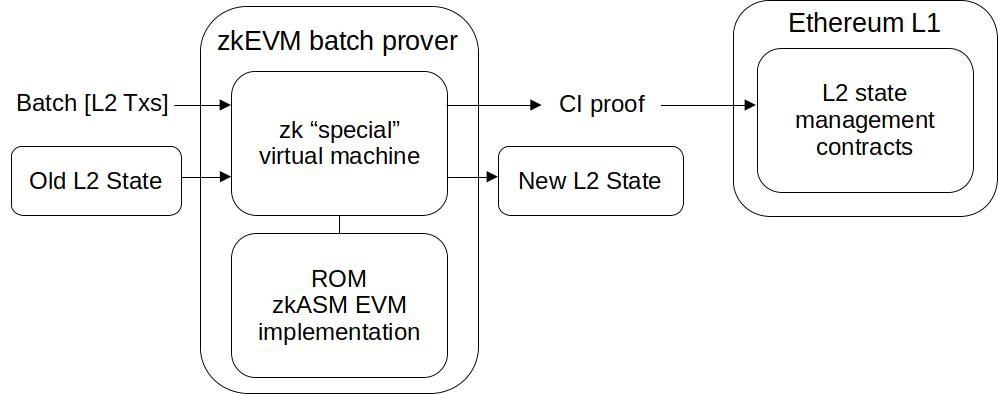
\includegraphics[width=0.8\columnwidth]{\assemblydir/figures/Introduction-schema}
\caption{zkEVM batch prover structure.}
\label{fig:hashk-add-bytes}
\end{figure}



In order to avoid futures misunderstood, it would be helpful to define and distinguish between the zkASM assembly instructions set and the EVM opcodes at this point.

\begin{itemize}
\item \textbf{zkASM instructions:} Set of instructions created and developed by Polygon to target a "special" zero-knowledge virtual machine that can execute computations with probable CI.
\item \textbf{EVM opcodes:} Set of instructions designed to target the EVM, used to define smart contract's computations.
\end{itemize}

Although zkASM instructions and EVM opcodes are different types of instructions, the Polygon zkEVM ROM contains a piece of code written in zkASM instructions to implement each EVM opcode.

%%%%%%%%%%%%%%%%%%%%%%%%%%%%%%%%%%%%%%%%%%%%%%%%%%%%%%%%%%%%%%%
\section{The ROM}
As explained above, the ROM is a zkASM program that can be executed by a  "special" virtual machine and allows to execute Polygon L2 State transitions with CI by inheriting Ethereum L1 security. This section aims to provide a detailed description of the ROM, allowing for a better understanding of its operation. The code of the ROM found at \href[]{https://github.com/0xPolygonHermez/zkevm-rom}{0xPolygonHermez/zkevm-rom} GitHub repository.


\subsection{ROM executions public parameters}

To achieve CI of a specific ROM execution, the resulting proof generated by the zkEVM batch prover must be successfully verified by L1 contracts. However, a zero-knowledge proof does not reveal any information about the specific computation being verified. Therefore, to allow the L1 smart to verify that a specific CI proofs corresponds to a specific state transition, a few "public" parameters of the computation are disclosed. The L1 verifier contract will verify the proof using this parameters and the verification will succeed only if the public parameters are those ones used to generate the proof by the prover. The disclosure of these parameters ensures that the proof being verified corresponds to a specific state transition, meaning that the execution of a specific batch over a specific state leads to a specific new state. L1 contracts provide data availability of the L2 batches, so that the prover is bound to on-chain data to fill the public parameters and generate a valid CI proof, and the verifier can access that data in a trustless manner during the proof verification.

The verification will succeed only if the public parameters match to those used to generate the CI proof by the prover. Each of the public parameters is listed and detailed below:


\begin{itemize}
	\item \textbf{oldStateRoot:} L2 State Merkle Root of the L2 State before the state transition that wants to be proven. Ensures the integrity of the old L2 State on which transactions are executed.
	\item \textbf{oldAccInputHash:} Unique cryptographic identifier of the previous batch in the batch chain, the batch whose execution led to the L2 state before the state transition that wants to be proven, ensures the correct position of the state transaction in the batches sequence.
	\item \textbf{oldBatchNum:} Unique batch index of the previous batch, the batch whose execution led to the L2 state before the state transition that wants to be proven.
	\item \textbf{newStateRoot:} L2 State Merkle Root of the L2 State after the state transition that wants to be proven. Ensures the integrity of the old L2 State that results of the state transition.
	\item \textbf{newAccInputHash:} Unique cryptographic identifier of the batch whose execution is being proved, ensures the integrity of the batch.
	\item \textbf{newBatchNum:} Unique batch index of the the batch whose execution is being proved.
	\item \textbf{localExitRoot:} L2 Bridge contract's Exit Merkle Tree(EMT) at the end of the batch execution, ensures the integrity of the bridging transactions going out form the L2. 
	\item \textbf{chainID:} Unique chain ID of Polygon zkEVM network, ensures that the computation can only be proven for a specific network.
	\item \textbf{forkID:} Unique identifier of the version of the ROM being used, ensures that the computation can only be proven for a specific version of the ROM code.
\end{itemize}

\subsection{ROM main.zkasm}
The  \href[]{https://github.com/0xPolygonHermez/zkevm-rom/blob/main/main/main.zkasm}{main.zkasm} is the zkASM code of the ROM where the batch processing and execution is described. The entry point of the ROM is represented by the \textbf{start} instruction. 

ROM's main.zkasm code is divided in the following 6 sections:
\begin{itemize}
	\item \textbf{A}: Load initial registers into memory.
	\item \textbf{B}: Set batch global variables.
	\item \textbf{C}: Loop parsing RLP transactions.
	\item \textbf{D}: Loop processing transactions.
	\item \textbf{E}: Batch asserts \& computations:.
	\item \textbf{F}: Finalize execution.
\end{itemize}

\subsubsection{A: Load initial registers into memory}

The ROM code describes a general computation to process and execute a batch of L2 transactions, but the specific batch to process must be given as well as all the values that can vary between different ROM executions. We refer to these values as ROM's input variables.

In the first lines of the ROM, all those inputs are loaded into the memory to be used later. Note that each input has a proper memory variable to be stored.


\begin{zkasm}
STEP => A
0                                   :ASSERT ; Ensure it is the beginning of the execution

CTX                                 :MSTORE(forkID)
CTX - %FORK_ID                      :JMPNZ(failAssert)

B                                   :MSTORE(oldStateRoot)
C                                   :MSTORE(oldAccInputHash)
SP                                  :MSTORE(oldNumBatch)
GAS                                 :MSTORE(chainID)

${getGlobalExitRoot()}              :MSTORE(globalExitRoot)
${getSequencerAddr()}               :MSTORE(sequencerAddr)
${getTimestamp()}                   :MSTORE(timestamp)
${getTxsLen()}                      :MSTORE(batchL2DataLength) ; less than 300.000 bytes. Enforced by the smart contract

B => SR ;set initial state root

; Increase batch number
SP + 1                              :MSTORE(newNumBatch)
\end{zkasm}

The first four lines ensure that this fragment of code is only executed at the beginning of the execution, i.e. they asserts that the \textbf{STEP} register is equal to 0, and that the version of the rom is correct, i.e ensures that the ROM's constant \textbf{FORK\_ID} equals to the \textbf{frok\_id} input variable. The following lines store the values of the input variables in memory variables. Note that most of them correspond to the execution's public parameters.

\subsubsection{B: Set batch gobal variables}

Batches are stored in Ethereum L1 following a specific data structure. The ROM uses the values in that data structure to identify the batch and ensure its integrity (refer to the technical documents regarding zkEVM state management to lean about batch data structure). The next section of the main.zkasm will load the batch data in the memory to be used later.

In the next three lines, the program will verify whether \textbf{globalExitRoot} is equal to 0. If it is, the execution flow will jump to the \textbf{skipSetGlobalExitRoot} line in the ROM. Note that the program first loads the value of \textbf{globalExitRoot} into register A and the value of 0 into register B before executing the combination of \textbf{EQ} and \textbf{JMPC(skipSetGlobalExitRoot)} instructions. The \textbf{EQ} instruction checks if A is equal to B, and if it is, the program flow will jump accordingly.

\begin{zkasm}
$${eventLog(onStartBatch, C)}

$ => A                                  :MLOAD(globalExitRoot)
0 => B
$                                       :EQ, JMPC(skipSetGlobalExitRoot)

\end{zkasm}

The section of main.zkasm shown below stores the \textbf{GlobalExitRoot} value in the \textbf{globalExitRootMap} of the \textbf{PolygonZkEVMGlobalExitRootL2.sol} contract instance, which allows users to claim bridged assets in L2 (refer to the technical documents regarding the zkEVM bridge). 0 is not a valid value for a \textbf{GlobalExitRoot}, therefore in this case, the previously explained jump will be executed and this part will be skipped. \textbf{globalExitRootMap} mapping entries has \textbf{GlobalExitRoot} as keys and the batch's timestamp as values.

\begin{zkasm}
setGlobalExitRoot:
0 => HASHPOS
$ => E                                  :MLOAD(lastHashKIdUsed)
E+1 => E                                :MSTORE(lastHashKIdUsed)

32 => D
A                                       :HASHK(E)
%GLOBAL_EXIT_ROOT_STORAGE_POS           :HASHK(E) ; Storage position of the global exit root map
HASHPOS                                 :HASHKLEN(E)
$ => C                                  :HASHKDIGEST(E)

%ADDRESS_GLOBAL_EXIT_ROOT_MANAGER_L2 => A
%SMT_KEY_SC_STORAGE => B

; read timestamp given the globalExitRoot
; skip overwrite timestamp if it is different than 0
; Since timestamp is enforced by the smart contract it is safe to compare only 32 bits in 'op0' with JMPNZ
$ => D                                  :SLOAD, JMPNZ(skipSetGlobalExitRoot)

$ => D                                  :MLOAD(timestamp)
$ => SR                                 :SSTORE ; Store 'timestamp' in storage position 'keccak256(globalExitRoot, 0)'
\end{zkasm}

Let's analyze the lines above in depth. Specific Solidity mapping values are stored in a specific contract storage slot computed as Keccak("key", "mapping slot"). Therefore, in order to compute the storage slot where the timestamp of a specific \textbf{globalExitRoot} will be stored, it is mandatory to perform a Keccak hash operation.

The first four lines are a consequence of how the hashes are performed in zkASM. First, the \textbf{HASPOS} register is set to zero in order to set the pointer of the hashing input array to its 0 position. Then, the \textbf{lastHashKIdUsed} memory variable is loaded into register E and incremented by one. \textbf{lastHashKIdUsed} contains the index of the last hash operation performed, therefore our hash operation will be next to it and the new value of register \textbf{E} will be used as its index.

The goal of line 6 is to set the length in bytes of the next entry in the hash input array that will be taken, by design from the register \textbf{D}. In this case, since both Keccak arguments are 32 bytes in length, the number 32 is set. In the following two lines, the two Keccak arguments are loaded into the hash inputs array: first, the \textbf{GlobalExitRoot} that was already in the \textbf{A} register, and then the slot address of the mapping in the contract's storage. Then, in line 9, the computation of the hash is triggered by giving \textbf{HASHPOS} as the length of the hash input array. Note that \textbf{HASHPOS} will be 64 since it auto-increments its value each time a byte is pushed into the hash input array via \textbf{HASHK} instruction, and we have pushed 32 bytes of \textbf{GlobalExitRoot} and 32 bytes of the slot address. In the following line the hash digest will be loaded to register C.

Next, in lines 12 and 13, the address of the \textbf{PolygonZkEVMGlobalExitRootL2.sol} contract instance and the type of Polygon zkEVM's state tree leaf that will contain the mapping value (3-Contract storage slot value) will be loaded into registers A and B, respectively. Note that at this moment, zkASM storage operations can be performed on the zkEVM state tree leaf that holds the 32-byte storage slot that corresponds to the value of the specific \textbf{GlobalExitRoot} in the mapping \textbf{globalExitRootMap} of the \textbf{PolygonZkEVMGlobalExitRootL2.sol} contract instance.

Line 18 will check if the storage slot is already set, i.e., if it is different from zero, and will skip lines 20 and 21 in that case to avoid overwriting a \textbf{GlobalExitRoot} that has already been set. Lines 20 and 21 will load the timestamp value from the memory variable to register D and then store it with the \textbf{SSTORE} instruction. Note that the \textbf{SR} is also updated with the latest Polygon zkEVM's state root value in the line 21.

The following 8 lines will save the previously computed state tree root to the memory variable batchSR. Then, they will load the number index of the last transaction executed in the L2 from the leaf that contains it in the state tree, and store it in the \textbf{txCount} memory variable.
\begin{zkasm}
skipSetGlobalExitRoot:
SR                                      :MSTORE(batchSR)
; Load current tx count
%LAST_TX_STORAGE_POS => C
%ADDRESS_SYSTEM => A
%SMT_KEY_SC_STORAGE => B
$ => D          :SLOAD
D               :MSTORE(txCount)
\end{zkasm}

TODO: EXPLAIN WHY MUST BE CHECKED THE KECCAK COUNTERS.

%%> Jesus Polygon:
%%Yep la idea es "demostrar" Que no tienes suficientes counters %%para seguir la ejecución
%%Y en ese caso, hacer las comprobaciones minimas y acabar la %%ejecución


\begin{zkasm}

; Compute necessary keccak counters to finish batch
$ => A          :MLOAD(batchL2DataLength)
; Divide the total data length + 1 by 136 to obtain the keccak counter increment.
; 136 is the value used by the prover to increment keccak counters
A + 1                                   :MSTORE(arithA)
136                                     :MSTORE(arithB), CALL(divARITH); in: [arithA, arithB] out: [arithRes1: arithA/arithB, arithRes2: arithA%arithB]
$ => B                                  :MLOAD(arithRes1)
; Compute minimum necessary keccaks to finish the batch
B + 1 + %MIN_CNT_KECCAK_BATCH => B      :MSTORE(cntKeccakPreProcess)
%MAX_CNT_KECCAK_F - CNT_KECCAK_F - B    :JMPN(handleOOCKatRLP)
\end{zkasm}



\subsubsection{C: Loop parsing RLP transactions}


In a batch, the transactions are represented as a byte array where each transaction is encoded using the Ethereum pre-EIP-115 or EIP-115 formats and following the RLP (Recursive-length prefix) standard. The encoded transaction is concatenated with the values v, r, and s of the signature. The section of main.zkasm that follows iterates through each transaction in the batch. For each transaction, a new zkasm memory context is created and the transaction data is parsed to extract the transaction values which are stored in memory variables for later use. Also each transaction data will be pushed to an specific keccak operation given by batchHashDataId  input buffer. The hash digest of all transaction data is used to calculate the accumulated hash of the batch in question.

The transactions must have one of the following structure:
\begin{itemize}
	\item EIP-155: rlp(nonce, gasprice, g asLimit, to, value, data, chainid, 0, 0,)vrs.
	\item pre-EIP-155: rlp(nonce, gasprice, gasLimit, to, value, data)vrs.
\end{itemize}



\begin{zkasm}
E+1 => E                            :MSTORE(lastHashKIdUsed)
0                                   :MSTORE(batchHashPos)
E                                   :MSTORE(batchHashDataId)
$ => A                              :MLOAD(lastCtxUsed)
A                                   :MSTORE(ctxTxToUse) ; Points at first context to be used when processing transactions

$${var p = 0}

txLoopRLP:
$ => A          :MLOAD(lastCtxUsed)
A+1 => CTX      :MSTORE(lastCtxUsed)

$ => A          :MLOAD(batchL2DataLength)
$ => C          :MLOAD(batchL2DataParsed)
C - A           :JMPN(loadTx_rlp, endCheckRLP)
endCheckRLP:
:JMP(txLoop)
\end{zkasm}

The first three lines will prepare the Keccak hash instance to compute the hash digest of all transaction data in the batch. It takes and stores in the memory a \textbf{batchHashDataId} based on the last hash ID used. Also, \textbf{batchHashPos} will be set to zero since it will be the pointer of the Keccak input that will be incremented with each transaction addition to the hash input.

Then the variable \textbf{ctxTxToUse} will be set to the last context used value to create new contexts ahead of older ones for each transaction in the batch.


The lines 9 to 15 are executed in a loop for each transaction in the batch. For each transaction, first, a new memory context will be created. The  variable \textbf{lastCtxUsed} will act as the loop index and will also give a specific context number to each transaction. Note that in each iteration, it will be incremented by 1. Then lines 13 to 15 will check if is the last iteration of the loop by comparing length of parsed batch with non parsed batch. In that case, the loop will break. If not, the \href[]{https://github.com/0xPolygonHermez/zkevm-rom/blob/main/main/load-tx-rlp.zkasm}{\textbf{loadTx\_rlp}} code will be executed, it can be found at the ROM's GitHub repository. It contains the logic to parse a transaction of the batch and store each transaction data value in a specific memory variable of the transaction's memory context. It also pushes the data to the hash of all transactions input.



\subsubsection{D: Loop processing transactions}

The section of main.zkasm that follows iterates again through all transactions in the batch, executing each one of them and applying the changes to the Polygon zkEVM state tree.
 
\begin{zkasm}
txLoop:
$ => A          :MLOAD(pendingTxs)
A-1 => A        :MSTORE(pendingTxs), JMPN(processTxsEnd)

$ => A          :MLOAD(ctxTxToUse) ; Load first context used by transaction
A+1 => CTX      :MSTORE(ctxTxToUse),JMP(processTx)

processTxEnd:
:CALL(updateSystemData)
processTxFinished:
$${eventLog(onFinishTx)}   :JMP(txLoop)

processTxsEnd:
\end{zkasm}

The lines 1 to 11 are executed in loop for each transaction. the variable \textbf{pendingTxs} will be the loop index. Note that now in each iteration it decrements by 1, starting from the last value set in the \textbf{pendingTxs} variable (for each transaction parsed by the former executed \textbf{loadTx\_rlp} code, the \textbf{pendingTxs} variable is incremented by one). Line 3 will check if all transactions in the batch are already processed by checking if the \textbf{pendingTxs} variable is less than 0. In that case, the loop will break. If not, the  \href[]{https://github.com/0xPolygonHermez/zkevm-rom/blob/main/main/process-tx.zkasm}{\textbf{process-tx}} code will be executed, it can be found at the ROM's GitHub repository. It contains the logic to process an Ethereum transaction adapted to Polygon zkEVM infrastructure. All the verifications that would be done in the Ethereum network, such as transaction signature verification, chain ID, etc., are also implemented in the \textbf{process-tx} code. Note that thanks to the former ROM's section (C), all transaction data can now be accessed through zkASM memory opcodes without the need to parse the bytes string of the batch's transactions again.

In each iteration of the loop, after processing a specific transaction, the subroutine \textbf{updateSystemData} is called (Line 9). Its code can be found on the ROM's GitHub repository in the \href[]{https://github.com/0xPolygonHermez/zkevm-rom/blob/main/main/utils.zkasm}{utils.zkasm} file. The system contract is a special contract in Polygon zkEVM L2 whose storage contains information about the network. The \textbf{updateSystemData} subroutine is meant to update the total processed transaction counter and the state root mapping in the system contract.

\subsubsection{E: Batch computations}

The section of main.zkasm that follows performs the last computations that have to be done for each batch.

First, it reads the \textbf{LocalExitRoot} of the \textbf{PolygonZkEVMGlobalExitRootL2.sol} contract instance and stores it in \textbf{newLocalExitRoot}, which is a variable meant to contain the computation public parameter \textbf{LocalExitRoot}. Since  \textbf{LocalExitRoot} is a public parameter, once the CI proof will be successfully verified by L1 contracts, this value will be sent to the \textbf{PolygonZkEVMGlobalExitRoot.sol} L1 contract instance to trigger the computation of the new bridge's Global exit root and enable to claim bridge transactions in L1.

\begin{zkasm}
;; Get local exit root
; Read 'localExitRoot' variable from GLOBAL_EXIT_ROOT_MANAGER_L2 and store
; it to the 'newLocalExitRoot' input
%ADDRESS_GLOBAL_EXIT_ROOT_MANAGER_L2  => A
%SMT_KEY_SC_STORAGE => B
%LOCAL_EXIT_ROOT_STORAGE_POS => C
$ => A                                          :SLOAD
A                                               :MSTORE(newLocalExitRoot)

\end{zkasm}

The next segment will ensure that the length of the input of the Keccak hash of all transaction data matches with the length of the byte array of the transactions given as computation input, i.e., all the transactions of given as computation input are included in the hash computation. Then computes the keccak hash and stores the hash digest in the \textbf{batchHashData} memory variable. This value will ensure the integrity of the batch's transactions data queried from L1.
 
\begin{zkasm}
;; Transactions size verification
; Ensure bytes added to compute the 'batchHashData' matches the number of bytes loaded from input
$ => A                          :MLOAD(batchHashPos)
$                               :MLOAD(batchL2DataLength), ASSERT

;; Compute 'batchHashData'
A => HASHPOS
$ => E                          :MLOAD(batchHashDataId)

HASHPOS                         :HASHKLEN(E)
$ => A                          :HASHKDIGEST(E)

A                               :MSTORE(batchHashData)
\end{zkasm}

The last segment will compute the accumulated hash of the batch and store it in the \textbf{newAccInputHash} variable, which is meant to contain the computation public parameter \textbf{newAccInputHash}. The accumulated hash will ensure the integrity of the batch data (transactions, timestamp, globalExitRoot) and that of all its predecessors, as well as the order in which they have been sequenced. The L1 verification contract will check that this value equals that one in its storage to ensure that the exact data queried from L1 has been used to perform the off-chain computations of the batch.

\begin{zkasm}
;; Compute 'newAccInputHash'
0 => HASHPOS

32 => D
$ => A                          :MLOAD(oldAccInputHash)
A                               :HASHK(0)

$ => A                          :MLOAD(batchHashData)
A                               :HASHK(0)

$ => A                          :MLOAD(globalExitRoot)
A                               :HASHK(0)

8 => D
$ => A                          :MLOAD(timestamp)
A                               :HASHK(0)

20 => D
$ => A                          :MLOAD(sequencerAddr)
A                               :HASHK(0)

HASHPOS                         :HASHKLEN(0)

$ => C                          :HASHKDIGEST(0)
C                               :MSTORE(newAccInputHash)
$${eventLog(onFinishBatch)}
\end{zkasm}



\subsubsection{F: Finalize execution}

The final section of main.zkasm will perform the final steps of ROM's execution, which is to load the values of computation results in the proper registers and set the initial values of some required registers. Then it will jump to the final wait. All of these steps are required to be in the code due to the system's design.

\begin{zkasm}
; Set output registers
$ => D                          :MLOAD(newAccInputHash)
$ => E                          :MLOAD(newLocalExitRoot)
$ => PC                         :MLOAD(newNumBatch)

; Set registers to its initials values
$ => CTX                        :MLOAD(forkID)
$ => B                          :MLOAD(oldStateRoot)
$ => C                          :MLOAD(oldAccInputHash)
$ => SP                         :MLOAD(oldNumBatch)
$ => GAS                        :MLOAD(chainID)
finalizeExecution:
:JMP(finalWait)
\end{zkasm}









%%%%%%%%%%%%%%%%%%%%%%%%%%%%%%%%%%%%%%%%%%%%%%%%%%%%%%%%%%%%%%%
\section{zkEVM Architecture}


\subsection{Registries}

In order to replicate the EVM opcodes, zkEVM introduces six state related generic registers named \A, \B, \C, \D and \E. However, since zkEVM operates over a finite field of almost 64 bits, each register is split into 8 limbs of 32 bits each: 
\begin{align*}
    &\A_0, \dots,  \A_7 \\
    &\B_0, \dots,  \B_7 \\
    &\C_0, \dots,  \C_7 \\
    &\D_0, \dots,  \D_7 \\
    &\E_0, \dots,  \E_7 \\
\end{align*}
with $\A_i, \B_i, \C_i, \D_i, \E_i \in \{0, \dots, 2^{32} - 1\}$. When storing a value in a register, the least significant bits are placed in the lowest limb, starting from the $0$-th one. That is, if we want to allocate a $32$ bits value in the \A-th register, we will fill only $\A_0$ with it. It we want to allocate a $64$ bits value, we will fill $\A_0$ and $\A_1$ and so on.  For example, if one want to store the value \texttt{0x12345678} in the \A register, the least significant byte \texttt{0x78} would be placed in $\A_0$ and the most significant byte \texttt{0x12} in $\A_3$. 

Apart from the generic registers related with the state of the zkEVM, there are additional registers in zkEVM that are used for various purposes. Here is a brief description of each of these registers:

\begin{itemize}
    
    \item \texttt{SR}: This is the status register and is used to indicate the current status of the processor. For example, it might indicate whether an arithmetic operation resulted in a carry or overflow, or whether an instruction encountered an error.
    
    \item \texttt{CTX}: This is the context register and is used to store the context of the current execution environment. For example, it might store information about the current smart contract being executed or the current transaction.
    
    \item \texttt{SP}: This is the stack pointer register and is used to point to the top of the stack. Every time a number is pushed onto the stack or removed from it, it is either increased or decreased. 
    
    \item \texttt{PC}: This is the EVM program counter register. The Program Counter (\texttt{PC}) encodes which instruction, stored in the code, should be next read by the EVM.  The program counter is usually incremented by one byte, to point to the following instruction, with some exceptions. For instance, the \texttt{PUSHx} instruction forces the \texttt{PC} to skip their parameter because it is longer than a single byte. The \texttt{JUMP} instruction modifies the program counter to a location determined by the top of the stack rather than increasing the \texttt{PC}'s value. 
    
    \item \texttt{GAS}: This is the gas register and is used to store the amount of gas remaining for the current transaction. Gas refers to the unit that measures the amount of computational effort required to execute specific operations on the Ethereum network.
    
    \item \texttt{RR}: This is the return register and is used to store the address to return to after a function call or jump.
    
    \item \texttt{zkPC}: This is the zkEVM program counter register. Similarly as explained in the \texttt{PC} register, it encodes which instruction of the zkEVM is being executed. This register will be crucial in order to ensure that the program that is being executed matches the program that wants to be proved. 
    
    \item \texttt{STEP}: This is the step register and is used to store the number of instructions executed so far in the current transaction.
    
    \item \texttt{MAXMEM}: This is the maximum memory register and is used to store the maximum amount of memory that can be allocated for the current transaction.
    
    \item \texttt{HASHPOS}: This is the hash position register and will contain the index of the next position of the bytes array of the input of the hash that we will start to fill. More information on that can be found in the hash-related instructions section. 
    
    \item \texttt{ROTL\_C}: This is the \C-rotate left (read-only) register and is used to flag a left rotation of the \C register by $4$ bytes. This has the effect of moving the $4$ most significant bytes of the \C register to the $4$ least significant bytes, and moving the $28$ least significant bytes to the $28$ most significant bytes. Later on, this rotated \C register can be assigned elsewhere. For example:
    
    \begin{zkasm}
        ROT_C + 2 => A
    \end{zkasm}
    increases by $2$ units the rotated value of \C and assigns it into the register \A.
    
    \item \texttt{RCX}: This is the repeat count register \texttt{RCX}, which is used in the repeat instruction. The repeat instruction allows for a certain instruction to be executed multiple times, based on the value stored in the \texttt{RCX} register. The \texttt{RCX} register is decremented by one each time the instruction is executed, until it reaches zero. The use of the \texttt{RCX} register in the repeat instruction allows for efficient execution of repetitive tasks, as it avoids the need for explicit loops in the code.
    
\end{itemize}

Each of these registers serves a specific purpose in the operation of zkEVM and is used by the various instructions and operations defined in the zkEVM specification.








\subsection{Binary} \label{sec:binary-sm}

The zkEVM contains a specific state machine in order to perform several $256$-bits operations. Each one of them are programmed in order to operate between the registers \A and \B. The implemented operations are the following:

\begin{itemize}
    
    \item \ADD ($+$). This operation adds two 256-bit strings. Invoked using \texttt{:ADD} instruction. 
    
    \item \SUB ($-$). This operation subtracts two 256-bit strings. Invoked using \texttt{:SUB} instruction. 
    
    \item \LT ($<$). This operation checks if a 256-bit string is smaller than another 256-bit string considering a codification of the binary strings without sign. Invoked using \texttt{:LT} instruction. 
    
    \item \SLT ($<$). This operation checks if a 256-bit string is smaller than another 256-bit string but considering a codification of the binary strings with sign (the codification used by the EVM is complement to two). Invoked using \texttt{:SLT} instruction. 
    
    \item \EQ ($=$). This operation checks if two 256-bit strings are equal. Invoked using \texttt{:EQ} instruction. 
    
    \item \AND ($\land$). This operation computes the bit-wise ``add" of the two strings. Invoked using \texttt{:AND} instruction. 
    
    \item \OR ($\lor$). This operation computes the bit-wise ``or" of the two strings. Invoked using \texttt{:OR} instruction. 
    
    \item \XOR ($\oplus$). This operation computes the bit-wise ``xor" of the two strings. Invoked using \texttt{:XOR} instruction. 
    
\end{itemize}

To understand how the \ADD, \SUB, \LT and \SLT operations work, we need to understand in first place how the EVM codes $256$-bit strings to signed and unsigned integers. Figure \ref{fig:3-bit-strings} shows these codifications for 3-bit strings but the idea can be easily extended to 256-bit strings.

\begin{figure}[h!]
    \centering
    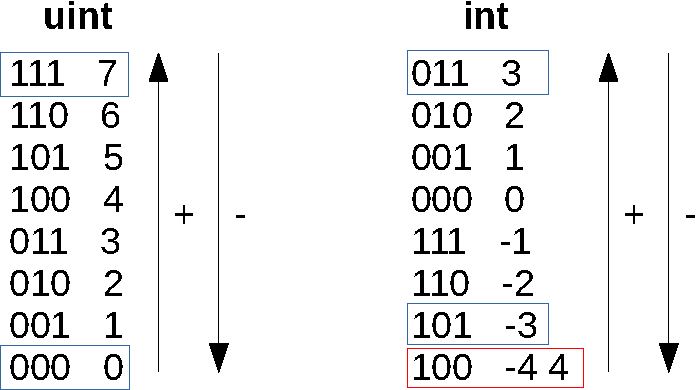
\includegraphics[width=0.55\textwidth]{../figures/integers_complement_two}
    \caption{Codifications of 3-bit strings for signed and unsigned integers as used by the EVM. \label{fig:3-bit-strings}}
\end{figure}


Adding two strings is performed bit by bit using the corresponding carry. For example, let's add the 3-bit strings $\texttt{0b001}$ and $\texttt{0b101}$:

\begin{itemize}
    
    \item We start with an initial $\texttt{carry}=0$ and adding the least significant bits: 
    
    $1+1+\texttt{carry}=1+1+0=0$ with the next carry being equal to $1$.
    \item Then, we add the next bits using the previous carry: 
    
    $0+0+\texttt{carry} = 0+0+1 = 1$ with the next carry being equal to $0$.
    \item Finally, we add the most significant bits: 
    
    $0+1+\texttt{carry}=0+1+0=1$ with the final carry being equal to $0$.
    \item As a result: $\texttt{0b001} + \texttt{0b101} = \texttt{0b110}$ with $\texttt{carry}=0$.
    
\end{itemize}

The sum $\texttt{0b001} + \texttt{0b101} = \texttt{0b110}$, for unsigned integers is $1+5=6$, while for signed integers encoded with complement to two this sum is $1+(-3) =(-2)$. In other words, we can do the same binary sum for both signed integers and for unsigned integers.

The operations \LT and \SLT are different however. When comparing unsigned integers (LT), the natural order for comparisons is applied, e.g. 110 (6) > 010 (2). When comparing signed integers (\SLT), we must take into account the most significant bit that acts as the sign. If the most significant bit of the two strings being compared is the same, the the natural order applies, e.g. 110 (-2) > 101 (-3). However, if the strings being compared have a different most significant bit, then the order must be flipped (bigger numbers start with 0), e.g. 001 (1) > 110 (-2). Finally, notice that with unsigned integers, there is a caveat since 4 and -4 have the same codification.

On the other hand, the \AND, \OR and \XOR operations are bit-wise operations, that is to say, the operation is done bit by bit. As a result, there are not any carries to be considered when operating a pair of bits. As we will see, this is going to make the checks easier to implement for bit-wise operations. Table \ref{tab:truth-tables} depicts the truth tables of \AND, \OR and \XOR operators, respectively.

\begin{figure}[h!]
    \[
    \begin{array}{|c|c|c|}
        \hline
        A 	&B 		&A \land B 	\\
        \hline
        0 	&0 		&0 				\\
        0 	&1 		&0				\\
        1 	&0 		&0 				\\
        1 	&1 		&1 				\\
        \hline
    \end{array}
    \hspace{0.5cm}
    \begin{array}{|c|c|c|}
        \hline
        A 	&B 		&A \lor B 	\\
        \hline
        0 	&0 		&0 				\\
        0 	&1 		&1				\\
        1 	&0 		&1 				\\
        1 	&1 		&1 				\\
        \hline
    \end{array}
    \hspace{0.5cm}
    \begin{array}{|c|c|c|}
        \hline
        A 	&B 		&A \oplus B 	\\
        \hline
        0 	&0 		&0 				\\
        0 	&1 		&1				\\
        1 	&0 		&1 				\\
        1 	&1 		&0 				\\
        \hline
    \end{array}
    \]
    \caption{Truth Tables of bit-wise operations}
    \label{tab:truth-tables}
\end{figure}

Notice that we do not consider the \texttt{NOT} operation. This is because the \texttt{NOT} operation can be easily implemented with the \XOR operation just by taking the 256-bit string and doing an \XOR with \texttt{0xff...ff}.



%TODO for Marc
\subsection{Arithmetic} \label{sec:arith-sm}


The Arithmetic State Machine (SM) is one of the six secondary state machines receiving instructions from the \textbf{Main SM} Executor. The main purpose of the Arithmetic State Machine is carry out elliptic curve arithmetic operations, such as Point Addition and Point Doubling as well as $256$-bits modular operations. The selected curve $E$ is the one with equation $y^2 = x^3 + 7$ over the field $\FF_p$ with:
\[
p = 2^{256} - 2^{32} - 2^9 - 2^8 - 2^7 - 2^6 - 2^4 - 1.
\] 

More specifically, thee Arithmetic SM is responsible for the execution of the following operations:

\begin{itemize}
    
    \item \textbf{Field Arithmetic}:  Here, $y_2$ and $y_3$ are the result of performing field arithmetic over $x_1,y_1$ and $x_2$. That is:
    
    \begin{equation}
        x_1 \cdot y_1 + x_2 = y_2 \cdot 2^{256} + y_3. \label{eq:field-arith}
    \end{equation}
    
    Note that if $y_1$ is set to $1$ then Eq. \eqref{eq:field-arith} represents field addition, and similarly if $x_2$ is set to $0$ then Eq. \eqref{eq:field-arith} represents field multiplication.
    
    \item \textbf{Elliptic Curve Addition}: Given two points $P = (x_1,y_1), Q = (x_2,y_2)$ from $E$ with $x_1 \neq x_2$, the point $P+Q = (x_3,y_3)$ is computed as follows:
    
    \begin{align*}
        x_3 &= s^2 - x_1 - x_2, \\
        y_3 &= s (x_1 - x_3) - y_1.
    \end{align*}
    
    where:
    \[
    s = \frac{y_2 - y_1}{x_2 - x_1}
    \]
    
    \item \textbf{Elliptic Curve Doubling}: Given a point $P = (x_1,y_1)$ from $E$ such that $P \neq \mathcal{O}$, the point $P+P = 2P = (x_3,y_3)$ is computed as follows:
    \begin{align*}
        x_3 &= s^2 - 2x_1, \\
        y_3 &= s (x_1 - x_3) - y_1.
    \end{align*}
    where:
    \[
    s = \frac{3x_1^2}{2y_1}.
    \]
    
\end{itemize}

Motivated by the implemented operations, the Arithmetic SM is composed of $6$ registers $x_1,y_1,x_2,y_2,x_3,y_3$. Each of these registers is decomposed in $16$ sub-registers of $16$-bit ($2$ byte) capacity, making a total of $256$ bits per register. We also need to provide $s$ and $q_0,q_1,q_2$, which are also elements of (the finite field) $256$ bits. 

The Arithmetic State Machine, combined with the Binary State Machine is used to implement opcodes like \textbf{signed and unsigned integer division}, \textbf{signed and unsigned module reducing}, \textbf{modular operations} or \textbf{exponentiation}. 







\subsection{Keccak-Related State Machines}


The KECCAK State Machine is in charge of validating the correct computation of EVM's KECCAK-256 hash. Unlike POSEIDON, due to its bit-wise nature, it is very inneficient in our set up and, therefore, it has been the focus for performing several optimizations. The strategy taken it is to use its circuit-like construction together with a PLONK-ish design in order to perform several KECCAK-f permutations at the same time. This State Machine is a complex one, because it has to deal with the Sponge Construction byte-wise and, later on, translate this execution bit-wise in order to compute all the KECCAK-f permutations in a parallel way. 

\subsubsection*{Sponge Construction}

The \textbf{sponge construction} is a simple iterated construction for building a function 
\[
F: \ZZ_2^* \to \ZZ_2^l
\] 
with variable-length input and arbitrary output length based on a fixed-length permutation
\[
f: \ZZ_2^b \to \ZZ_2^b
\] 
operating on a fixed number $b$ of bits. Here $b$ is called the \textbf{width}. The array of $b$ bits that $f$ keeps transforming is called the \textbf{state}. The state array is split in two chunks of $r$ and $c$ bits respectively. We call $r$ the \textbf{bitrate} (or rate) and $c$ the \textbf{capacity}. We will understand later on the motivation for this splitting. 

Let us describe how the sponge construction works:

\begin{enumerate}
    
    \item First of all, the input string is padded with a reversible \textbf{padding rule}, in order to achieve a length divisible by $r$. Subsequently, it is cut into blocks of $r$ bits. We also initialize the $b$ bits of the state to zero. 
    
    \item (\textit{Absorbing Phase}) In this phase, the $r$-bit input blocks are XORed into the first $r$ bits of the state, interleaved with applications of the function $f$. We proceed until processing all blocks of $r$-bits. Observe that the last $c$ bits corresponding to the capacity value does not absorb any input from the outside. 
    
    \item (\textit{Squeezing Phase}) In this phase, the first $r$ bits of the state are returned as output blocks, interleaved with applications of the function $f$. The number of output blocks is chosen at will by the user. Observe that the last $c$ bits corresponding to the capacity value are never output during this phase. Actually, if the output exceeds the specified length, we will just truncate it in order to fit. 
    
\end{enumerate}

We depict an schema of the sponge construction in Figure \ref{fig:sponge-construction}. 

\begin{figure}[H]
    \centering
    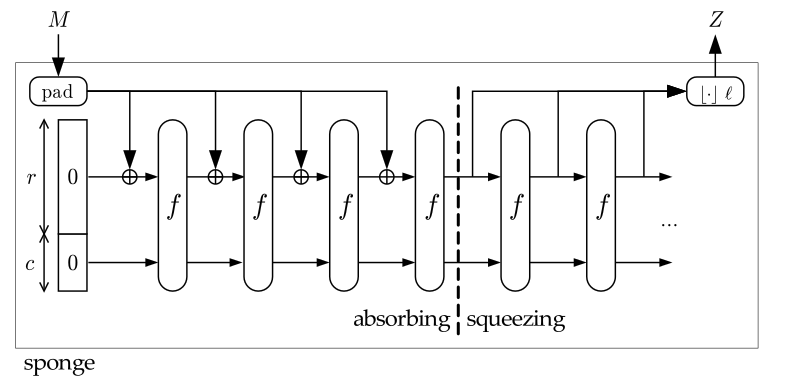
\includegraphics[width=0.6\columnwidth]{../figures/sponge-construction}
    \caption{Schema of Sponge Construction.}
    \label{fig:sponge-construction}
\end{figure}

The elements that completely describe a single instance of a sponge construction are: the fixed-length permutation $f$, the padding rule $\mathbf{pad}$ and the rate value $r$. 

\subsubsection*{EVM Hash Function Specification}

The EVM makes use of KECCAK-256 hash function, which is constructed using KECCAK$[512]$ sponge construction. Let us, therefore, define the KECCAK$[c]$ sponge construction. This sponge operates with a width of $1600$ bits and a rate of $1600 - c$. In the case of KECCAK$[512]$, the rate chunk is composed of $1088$ bits (or equivalently, $136$ bytes) and the capacity chunk has $512$ bits (or equivalently, $64$ bytes). The permutation used in KECCAK$[c]$ is KECCAK-$p[1600, 24]$ (See \cite{bertoni2013keccak}). The last ingredient we need to define in order to completely specify the hash function is the padding rule. In KECCAK$[c]$, the padding pad10*1 is used. If we define $j = (-m-2) \mod{r}$, where $m$ is the length of the input in bits, then the padding we have to append to the original input message is 
\[
P = 1 \mid\mid 0^j \mid\mid 1.
\]
Thus, given an input bit string $M$ and a output length $d$, KECCAK$[c](M, d)$ outputs a $d$ bit string following the previous sponge construction description. 

It should be noted that this construction does \textbf{not} follow the FIPS-202 based standard (a.k.a SHA-3). According to \cite{sha3standard}, NIST changed the SHA3 padding to
\[
\text{SHA3-256}(M) = \text{KECCAK}[512](M \mid\mid 01, 256).
\]
The difference is the additional $01$ bits appended to the original message, which were not present in the orignal KECCAK specification. 


\subsubsection*{zkEVM Keccak-related State Machines Pipeline}

Unlike the other state machines previously explained, rather than implementing the Keccak-256 hash function as a single state machine, the zkEVM does so in a framework of four state machines. They are as follows:

\vspace{3mm}
\begin{figure}[H]
    \centering
    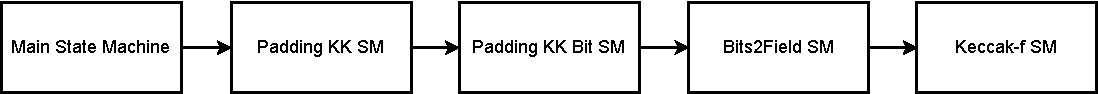
\includegraphics[width=0.9\columnwidth]{../figures/keccak-sm.drawio}
    \caption{Pipeline for Keccak-related State Machines.}
    \label{fig:keccak-sm}
\end{figure}

\begin{itemize}
    
    \item The \textbf{Padding KK} SM is used for padding purposes, as well as validation of hash-related computations pertaining to the \textbf{Main SM}'s queries. As depicted in the above figure, the \textbf{Padding KK SM} is \textbf{Main SM}'s gateway to the Keccak hashing state machines.
    
    \item The \textbf{Padding KK Bit} SM converts between two string formats, the bytes of the \textbf{Padding KK SM} to the bits of the \textbf{Keccak-f SM}, and vice-versa.
    
    \item The \textbf{Bits2Field SM} is used specifically for parallelizing \textbf{Keccak-f SM} implementation. It acts as a multiplexer between the \textbf{Padding KK Bit SM} and the \textbf{Keccak-f SM}. This state machine is called \textbf{Bits2Field} because it initially ensured the correct packing of bits from 4444 different blocks of the \textbf{Padding KK Bit SM} into a single field element.
    
    \item The \textbf{Keccak-F SM} computes string hashes at the request of the \textbf{Main SM}. Although the \textbf{Keccak-f SM} is a binary circuit, it operates on a 44bits-by-44bits basis rather than a bit-by-bit basis. This equates to running four 4444 hashing circuits in parallel.
    
\end{itemize}

\subsection{Poseidon-Related State Machines}

The \textbf{Poseidon State Machine} is a secondary state machine that receives instructions from the \textbf{Main State Machine} of the zkProver. It uses the Poseidon hash function to generate hash values in response to requests from the \textbf{Storage SM} (which we will see later on) and instructions from the \textbf{Main SM} Executor. Poseidon Actions are the directives that the \textbf{Poseidon SM} receives from one of the two SMs. It performs the Poseidon Actions as a secondary SM and also verifies that the output hash values were accurately calculated.


Poseidon (See \cite{poseidon}) is a hash function designed to minimize prover and verifier complexities when zero-knowledge proofs are generated and validated. The previously defined KECCAK-256 cryptographic hash require large circuits as they are not tailored to finite fields used in ZK proof systems (actually, KECCAK-256 works well in binary fields, and we will see later on that this fact introduces a lot of complexity in the constrain design). For this reason, zkEVM uses Poseidon hash as the main internal hash function. 

More concretely, we will now specify the specific instance of Poseidon that zkEVM uses. We will work over the field $\FF_p$ where $p = 2^{64} - 2^{32} + 1$. The state width of the Poseidon permutation is of $8$ field elements (observe that we are changing the paradigm, working with whole field elements instead of working bit-wise) meanwhile we will work with a capacity of $4$-field elements. 

The permutation used in Poseidon is a round function. A typical round function consists of three operations; an addition of a round-key $ARC(\cdot)$, a non-linear function $S$ (i.e., a substitution box or S-box), and a linear function $L$ which is often an affine transformation (in particular, an MDS matrix $M$). Some rounds are partial rounds because they use only one S-box instead of the full number of S-boxes, one for each element of the state. For security purposes against certain cryptanalytic attacks, outer rounds are full rounds, while the inner rounds are partial rounds. 

Denote the number of rounds by $R=R_F+R_P$ where $R_F$​ is the number of full rounds and $R_P$ is the number of partial rounds. Also, let $M(\cdot)$ denote the linear diffusion layer. Then, the figure blow depicts the Poseidon's permutation. 

\begin{figure}[H]
    \centering
    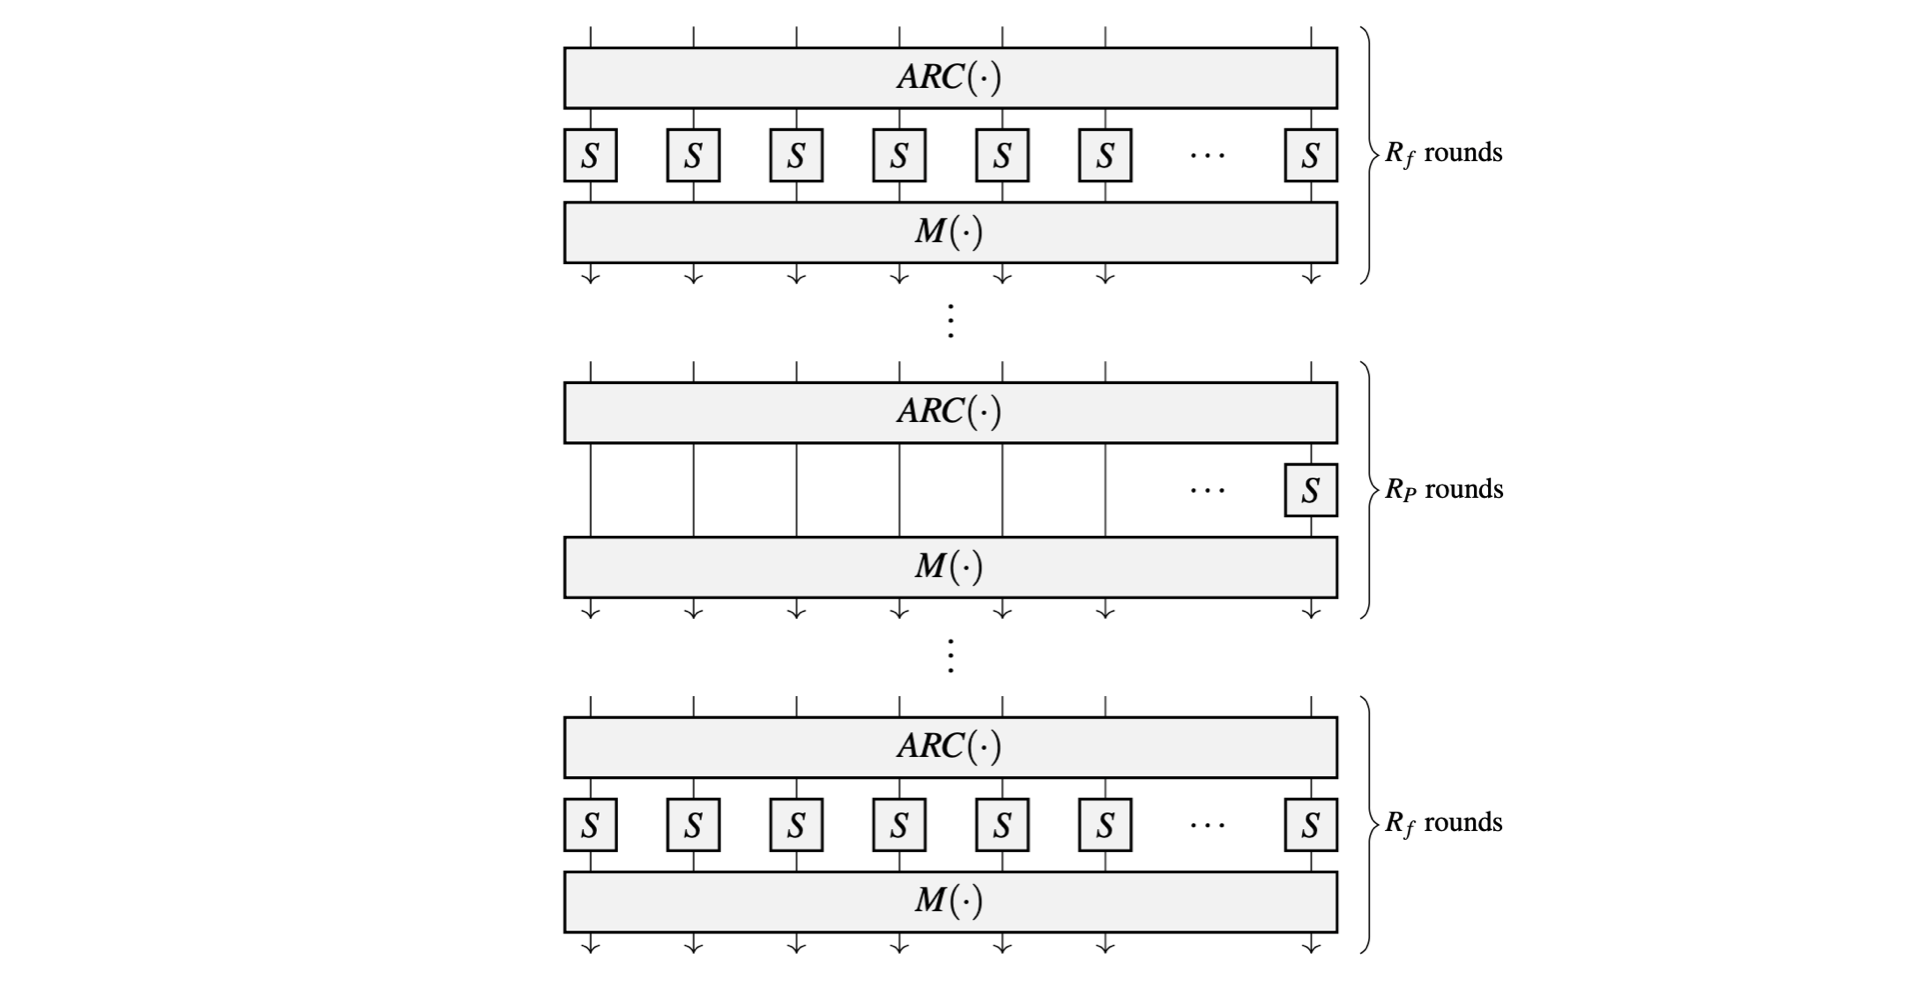
\includegraphics[width=\columnwidth]{../figures/poseidon-hades}
    \caption{HADES-based Poseidon's permutation.}
    \label{fig:poseidon-hades}
\end{figure}

The Poseidon S-box layer that we will use is the $7$-power S-Box, i.e.
\[
SB(x) = x^7,
\]
The Poseidon instance also requires to specify the number of full and partial rounds of the permutation. In our case, we will use 
\[
R_F = 8 \text{ (number of full rounds) }, \quad R_P = 22 \text{ (number of partial rounds)}
\]
Only one squeezing iteration will be effectuated, with an output of the first $4$ field elements of the state (which consists of approximately $256$-bits, but no more than that). The Round Constants and the MDS matrix are completely specified using the previous parameters. 



\subsection{Memory-Related State Machines}



\subsubsection*{Memory State Machine}


The memory of the EVM (Ethereum Virtual Machine) is a volatile read-write memory that
is used to store temporary data during the execution of transactions of smart contract functions. That is, data in memory is populated during transaction's execution but it does not persist between transactions. The memory is an array of $256$-bit ($32$ bytes) words that can be accessed through \textit{addresses at byte level}, that is to say, each byte in the memory has a different address. Memory has addresses of $32$ bits and initially, all memory locations are composed by bytes set to zero. Now, let's see the layout in memory of the following two words 0xc417...81a7 and 0x88d1...b723. Table \ref{tab:first-example} shows this layout.

\begin{figure}[h!]
    \[
    \begin{array}{|c|c|}
        \hline
        \mathbf{ADDRESS} &\mathbf{BYTE} \\ \hline
        \mathtt{0} &\mathtt{0xc4} \\
        \mathtt{1} &\mathtt{0x17} \\
        \mathtt{\vdots} &\mathtt{\vdots} \\
        \mathtt{30} &\mathtt{0x81} \\
        \mathtt{31} &\mathtt{0xa7} \\
        \mathtt{32} &\mathtt{0x88} \\
        \mathtt{33} &\mathtt{0xd1} \\
        \mathtt{\vdots} &\mathtt{\vdots} \\
        \mathtt{62} &\mathtt{0xb7} \\
        \mathtt{63} &\mathtt{0x23} \\
        \hline
    \end{array}
    \]
    \caption{Layout in memory of \texttt{0xc417...81a7} and \texttt{0x88d1...b723}.}
    \label{tab:first-example}
\end{figure}

Observe that each word has 32 bytes and that the words are stored in Big-Endian form, i.e. the most significant bytes are set in the lower addresses. The EVM provides three opcodes to interact with the memory area. We have an opcode to read and an opcode to write 32-byte words providing an offset:

\begin{itemize}
    
    \item \MLOAD: It receives an offset and returns the 32 bytes in memory starting at that offset.
    
    \item \MSTORE: It receives an offset and saves 32 bytes from the offset address of the memory.
    
\end{itemize}

Considering our previous memory contents, if we perform an \MLOAD with an offset of \texttt{1}, we would obtain the following word: \texttt{0x17...a788}. On the other hand, if we do an \MSTORE with an offset of \texttt{1} with the word \texttt{0x74f0...ce92}, we would modify the content of the memory as shown in Table \ref{tab:second-example}. 

\begin{figure}[h!]
    \[
    \begin{array}{|c|c|}
        \hline
        \mathbf{ADDRESS} &\mathbf{BYTE} \\ \hline
        \mathtt{0} &\mathtt{0xc4} \\
        \mathtt{1} &\mathtt{\textbf{0x74}} \\
        \mathtt{2} &\mathtt{\textbf{0xf0}} \\
        \mathtt{\ldots} &\mathtt{\ldots} \\
        \mathtt{31} &\mathtt{\textbf{0xce}} \\
        \mathtt{32} &\mathtt{\textbf{0x92}} \\
        \mathtt{33} &\mathtt{0xd1} \\
        \mathtt{\ldots} &\mathtt{\ldots} \\
        \mathtt{62} &\mathtt{0xb7} \\
        \mathtt{63} &\mathtt{0x23} \\
        \hline
    \end{array}
    \]
    \caption{Layout in memory after the introduction of \texttt{0x74f0...ce92}.}
    \label{tab:second-example}
\end{figure}

When the offset is not a multiple of 32 (or \texttt{0x20}), as in the previous example, we have to use bytes from two different words when doing \MLOAD or \MSTORE.

Finally, the EVM provides a write memory operation that just writes a byte:

\begin{itemize}
    
    \item \MSTOREE: It receives an offset and saves one byte on that address of the memory.
    
\end{itemize}

Notice that \MSTOREE always uses only one word.

The \textbf{Memory SM} is in charge of proving the memory operations in the execution trace. As mentioned, read and write operations use addresses at byte level in the EVM. However, doing the proofs byte by byte would consume many values in the trace of this state machine.

Instead, in this machine, we operate addressing words (32 bytes). For example, if we have the memory layout from Table \ref{tab:first-example}, then we would have the memory layout of Table \ref{tab:third-example} with addresses that point to 32-byte words.

\begin{figure}[h!]
    \renewcommand{\figurename}{Table}
    \[
    \begin{array}{|c|c|}
        \hline
        \textbf{ADDRESS} & \textbf{32-BYTE WORD} \\ \hline
        \mathtt{0} &\mathtt{0xc417...81a7} \\
        \mathtt{1} &\mathtt{0x88d1...b723} \\
        \hline
    \end{array}
    \]
    \caption{Layout in the memory state machine.}
    \label{tab:third-example}
\end{figure}

The \textbf{Memory SM} uses this latter layout, the 32-byte word access, to check reads and writes. However, as previously mentioned, the EVM can read and write with offsets at a byte level. As a result, we will need to check the relationship between byte access and 32-byte word access. For these checks, we have another state machine called \textbf{Memory Align SM} that is discussed below.


\subsubsection*{Memory Align State Machine} 



The \textbf{Memory SM} checks memory reads and writes using a 32-byte word access, while
the EVM can read and write 32-byte words with offsets at a byte level.
Table \ref{tab:byte:32byte:example} shows an example of possible byte-addressed and 32-byte-addressed memory layouts for the same content (three words).

\begin{figure}[h!]
    \renewcommand{\figurename}{Table}
    \[
    \begin{array}{|c|c|}
        \hline
        \mathbf{ADDRESS} &\mathbf{BYTE} \\ \hline
        \mathtt{0x00} &\mathtt{0xc4} \\
        \mathtt{0x01} &\mathtt{0x17} \\
        \mathtt{0x02} &\mathtt{0x4f} \\
        \mathtt{\ldots} &\mathtt{\ldots} \\
        \mathtt{0x1e} &\mathtt{0x81} \\
        \mathtt{0x1f} &\mathtt{0xa7} \\
        \hline
        \mathtt{0x20} &\mathtt{0x88} \\
        \mathtt{0x21} &\mathtt{0xd1} \\
        \mathtt{0x22} &\mathtt{0x1f} \\
        \mathtt{\ldots} &\mathtt{\ldots} \\
        \mathtt{0x3e} &\mathtt{0xb7} \\
        \mathtt{0x3f} &\mathtt{0x23} \\
        \hline
        \mathtt{0x40} &\mathtt{0x6e} \\
        \mathtt{0x41} &\mathtt{0x21} \\
        \mathtt{0x42} &\mathtt{0xff} \\
        \mathtt{\ldots} &\mathtt{\ldots} \\
        \mathtt{0x5e} &\mathtt{0x54} \\
        \mathtt{0x5f} &\mathtt{0xf9} \\
        \hline
    \end{array}
    \]
    \[
    \begin{array}{|c|c|}
        \hline
        \mathbf{ADDRESS} &\mathbf{32-BYTE~~WORD} \\ \hline
        \mathtt{0x00} &\mathtt{0xc4174f...81a7} \\
        \hline
        \mathtt{0x01} &\mathtt{0x88d11f...b723} \\
        \hline
        \mathtt{0x02} &\mathtt{0x6e21ff...54f9} \\
        \hline
    \end{array}
    \]
    \caption{Sample memory layouts for byte and 32-byte access.}
    \label{tab:byte:32byte:example}
\end{figure}

The relationship between the $32$-byte word addressable layout and the byte addressable layout is called ``memory alignment" and the \textbf{Memory Align SM} is the state machine that checks the correctness of this relationship. Notice that, in the general case, \MLOAD operation requires reading bytes of two different words. Considering that the content of the memory is the one shown at Table \ref{tab:byte:32byte:example}, since the EVM is addressed at a byte level, if we want to check a read from the EVM of a word starting at the address \texttt{0x22}, the value that we should obtain is the following:
\[
\val = \mathtt{0x1f \cdots b7236e21}.
\]
We denote the content of the words affected by an EVM memory read as $\mF$ and $\mS$.
In our example, these words are the following:
\[
\mF = \mathtt{0x} \mathtt{88d11f} \cdots \mathtt{b723},
\quad \mS =  \mathtt{0x} \mathtt{6e21ff} \cdots \mathtt{54f9}.
\]
We define a read block as the string concatenating the content of the words affected by the read: $\mF \mid \mS$.
Figure \ref{fig:mload-ex} shows the affected read words $\mF$ and $\mS$ that form the affected read block 
and the read value \val for a read from the EVM at address \texttt{0x22} in our example memory of Table \ref{tab:byte:32byte:example}.

\begin{figure}[h!]
    \centering
    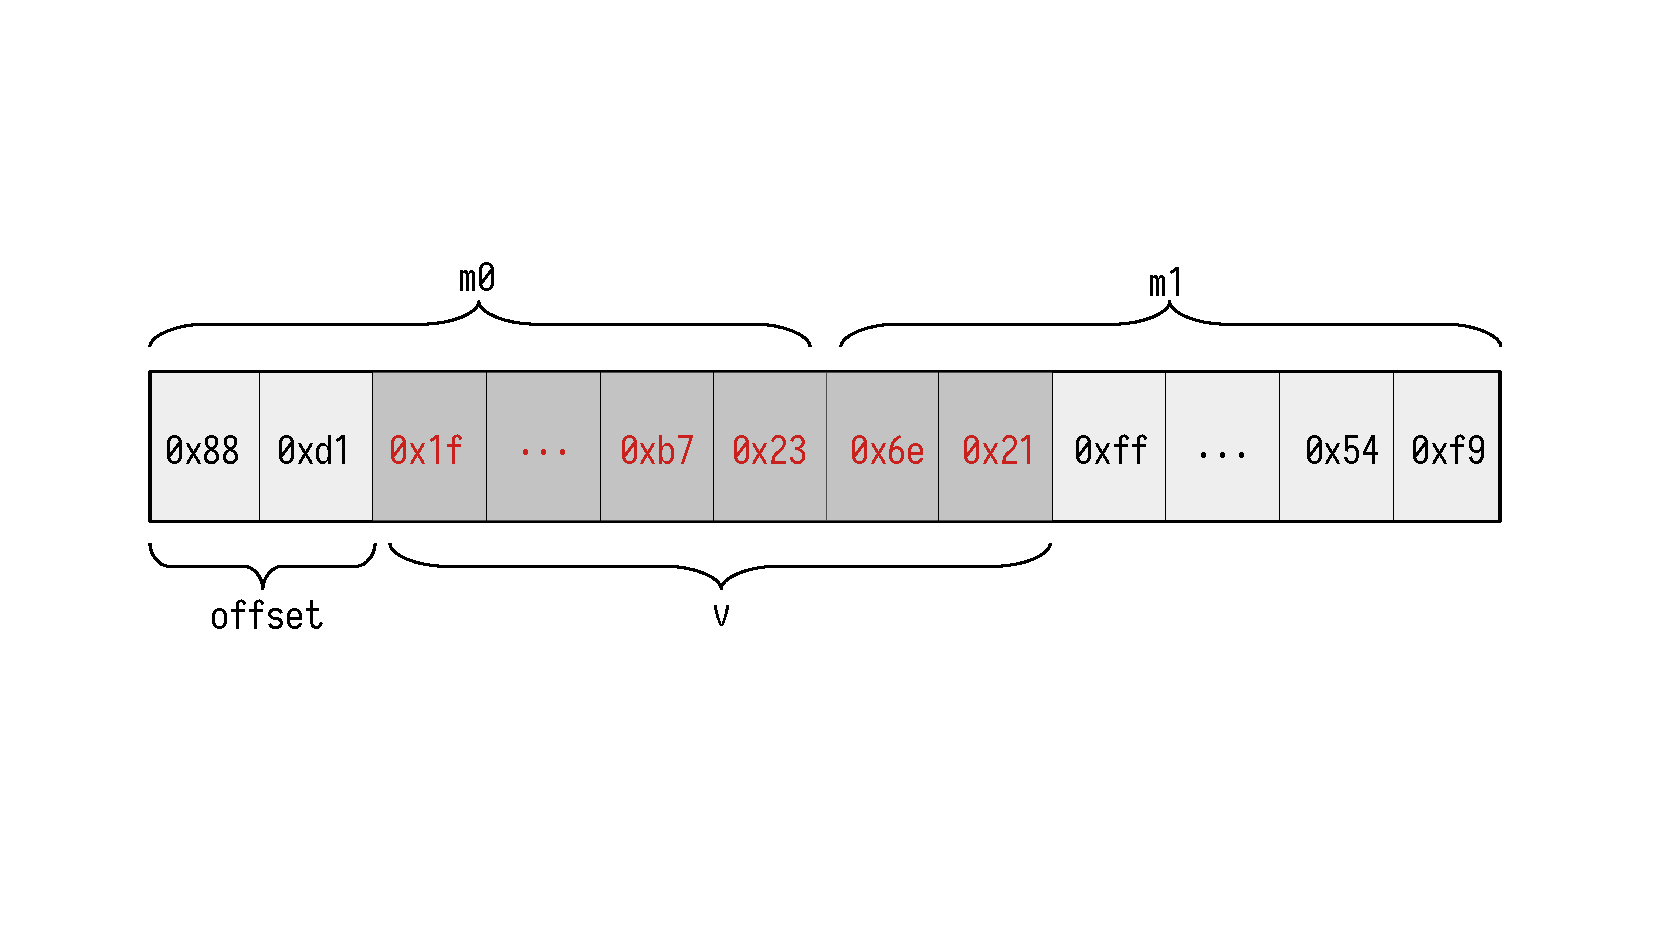
\includegraphics[width=1\columnwidth, trim=0 5cm 0 4cm, clip]{../figures/mload_ex}
    \caption{Schema of \MLOAD example.}
    \label{fig:mload-ex}
\end{figure}

Let us now introduce the flow at the time of validating a read. Suppose that we want to validate that if we perform an \MLOAD operation at the address $\mathtt{0x22}$, we get the previous value $\mathtt{0x1f\dotsb7236e21}$. At this point, the main state machine will perform several operations. First of all, it will have to query for the values \mF and \mS. Henceforth, it must call the \textbf{Memory SM} in order to validate the previous queries. 

Observe that it is easy to extract the memory positions to query from the address $\mathtt{0x22}$. In fact, if $a$ is the memory position of the \MLOAD operation, then \mF is always stored at the memory position $\lfloor \frac{a}{32} \rfloor$ and \mS is stored at the memory position $\lfloor \frac{a}{32} \rfloor + 1$. In our example, $a = \mathtt{0x22} = 34$. Hence, \mF is stored at the position $\lfloor \frac{32}{34} \rfloor = \mathtt{0x01}$ and \mS is stored at the position $\lfloor \frac{32}{34} \rfloor + 1= \mathtt{0x02}$. 

Secondly, we should extract the correct \offset. The \offset represents an index between $0$ and $31$ indicating the number of bytes we should offset from the starting of \mF to correctly place \val in the block. In our case, the \offset is $2$. Similarly as before, it is easy to obtain the offset from $a$. In fact, the it is equal to $a \mod{32}$. Now, the \textbf{Main SM} will check against the Memory Align State Machine that \val is a correct read given the affected words \mF and \mS and the \offset. That is, we should check that the value $\val$ can be correctly split into \mF and \mS using the provided \offset. 


Similarly, \MSTORE instruction requires, in general, writing bytes in two words.
The idea is very similar, but we are provided with a value \val that we want to write into a specific location of the memory. We will denote by \wF and \wS the words that arise from \mF and \mS after the corresponding write. 

Following our previous example, suppose that we want to write 
\[
\val = \mathtt{0xe201e6\dots662b}
\] 
in the address \texttt{0x22} of the byte-addressed Ethereum memory. We are using the same \mF and \mS (and since we are writting into the same address as before) and they will transition into  (see Figure \ref{fig:mstore-ex}):
\[
\wF = \mathtt{0x88d1}\color{-red!75}\mathtt{e201e6\dots}\color{black},\quad \wS =  \mathtt{0x}\color{-red!75} \mathtt{662b}\color{black} \mathtt{ff\dots54f9}.
\]

\begin{figure}[h!]
    \centering
    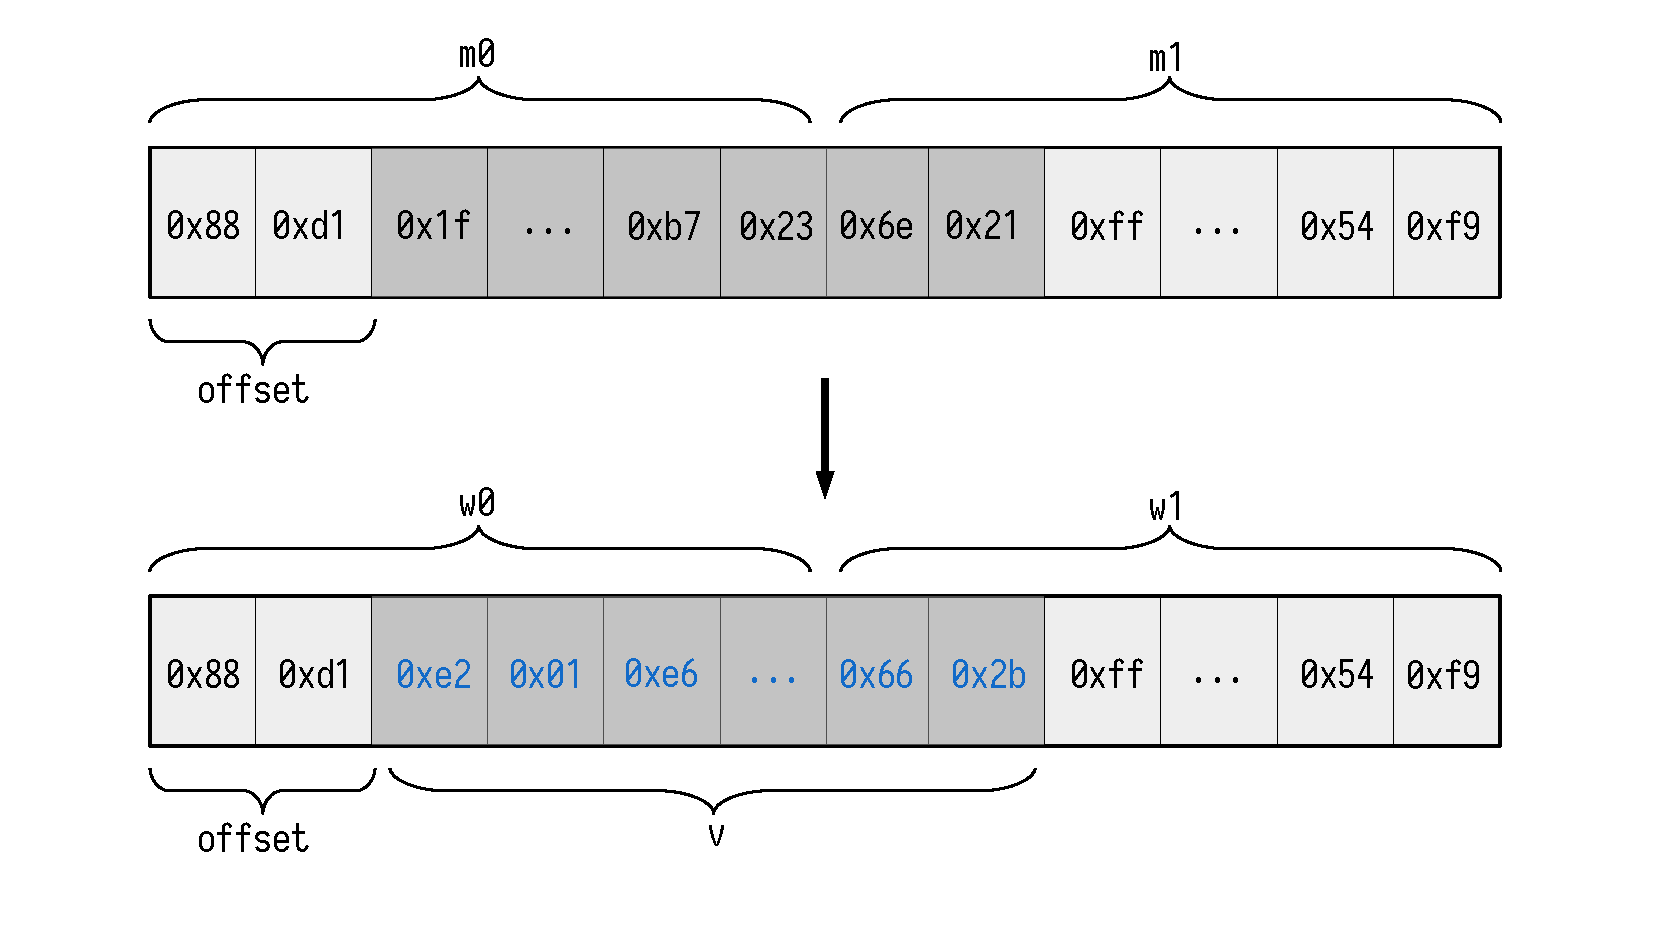
\includegraphics[width=1\columnwidth]{../figures/mstore_ex}
    \caption{Schema of \MSTORE example.}
    \label{fig:mstore-ex}
\end{figure}

Just as before, the main state machine will need to perform several operations. We will be given an address \addr, an offset value \offset and a value to be wrote \val. Identically as before, the \textbf{Main SM} will be in charge of reading the zkEVM memory to find \mF and \mS from the given address and offset. Of course, the validity of this query should be performed with a specific Plookup into the \textbf{Memory SM}, just as before. 

Now, the \textbf{Main SM} can compute \wF and \wS from all the previous values in a uniquely way. The way of validating that we are providing the correct \wF and \wS is to perform a Plookup into the \textbf{Memory Align SM}. That is, we will check that the provided values \wF and \wS are correctly constructed from the provided \val, \mF, \mS and \offset values. 


Finally, the last opcode \MSTOREE works similarly, \textit{but it only affects one word} \mF. Moreover, we can only write one byte and hence, only the less significant byte of \val will be considered into the write. Observe that, in this opcode, \mS and \wS are unconstrained.




\subsection{Storage SM}


The \textbf{Storage SM} is  in charge of validate operations over the key-value storage structure present in the EVM. The \textbf{Storage SM} is an essential building block for designing a more generic virtual machine that can check the correctness of state transitions resulting from executing smart contract transactions. The keys are expressed with 4 elements of $\FF_p$, while the values are expressed using 8 elements in $\FF_p$, where each of these eight elements have 0's at their most 32 significant bits.


The operations over the \textbf{Storage SM} are the typical Create, Read, Update and Delete (CRUD). A specific behavior of the \textbf{Storage SM} is that, in read operations, it returns zero if a key is not found. The structure used to build the key-value storage that can be proven with zero knowledge is a specific variant 
of a Merkle Patricia Tree (MPT).

In general, a Merkle tree is a data structure where every \emph{leaf} of the tree contains the cryptographic hash of a value and every \emph{non leaf}, which we also denote as \emph{branch}, contains the concatenated hashes of its children. Merkle trees allow to link a set of values to a unique hash called the \emph{root} of the tree and the efficient and secure verification of containment of large sets of key-values. In our case, we will use the key to unequivocally determine the position of the leaf in the Merkle tree. Furthermore, we are going to use the previously explained Poseidon hash function because it is a function that can be verified with zero-knowledge primitives in a more friendly way than other standard hash functions like KECCAK. Moreover, two different instances of Poseidon hash function (achieved modifying the initial value for the capacity) should be used for hashing leafs and branches to prevent possible attacks. 

The mechanics of the particular MPT proposed and its operations are described in detail later but essentially, proving operations over this hash structure involves to types of checks:

\begin{itemize}
    
    \item For read operations, we need to show that the value of a related key is included at the tree at the correct position.
    
    \item For write operations, we have to prove that modifications lead to the appropriate new root.
    
\end{itemize}




\subsection{Counters}

Counters are a mechanism to control that the total number of steps do not exceed the maximum polynomial size. The purpose of counters is to limit the number of steps that can be taken during the processing of a transaction, in order to ensure that the computation terminates within a certain time bound, defined by the polynomial size, currently stored in a constant

\begin{zkasm}
    CONST %TOTAL_STEPS = 2**23
\end{zkasm}
to prevent the cryptographic proof system from failing due to a denial-of-service attack. Additionally, it is important to consider that there is a fixed minimum number of steps required to complete the processing of a transaction:

\begin{zkasm}
    CONST %MIN_STEPS_FINISH_BATCH = 200 
\end{zkasm}

As a result, the total number of steps is determined by the following variable:

\begin{zkasm}
    CONST %MAX_CNT_STEPS = %TOTAL_STEPS - %MIN_STEPS_FINISH_BATCH
\end{zkasm}

Since there are operations that are more often used than others, it is a really good practice to limit the steps for each of the state machines individually. The values assigned to these counters are typically derived through a combination of design considerations and empirical testing. Design considerations may include factors such as the expected input rate or the maximum number of cycles the system can handle before failure. Empirical testing may involve running simulations or testing the system in a real-world environment to determine appropriate counter values.

\begin{zkasm}
    CONST %MAX_CNT_ARITH = %TOTAL_STEPS / 32
    CONST %MAX_CNT_BINARY = %TOTAL_STEPS / 16
    CONST %MAX_CNT_MEM_ALIGN = %TOTAL_STEPS / 32
    CONST %MAX_CNT_KECCAK_F = (%TOTAL_STEPS / 155286) * 44
    CONST %MAX_CNT_PADDING_PG = (%TOTAL_STEPS / 56)
    CONST %MAX_CNT_POSEIDON_G = (%TOTAL_STEPS / 30)
\end{zkasm}




















%%%%%%%%%%%%%%%%%%%%%%%%%%%%%%%%%%%%%%%%%%%%%%%%%%%%%%%%%%%%%%%
\section{zkASM Language}



%%%%%%%%%%%%%%%%%%%%%%%%%%%%%%%%%%%%%%%%%%%%%%%%%%%%%%%%%%%%%%%

\subsection{Basic Syntax}

This section is devoted to explain the basic syntax of zkASM from a high-level point of view. Advanced syntax is totally dependent of the use case (e.g. the design of a zkEVM) and will be explained in more detail with more complete examples in a latter section.

It is important to remark that each instruction of the zkASM is executed sequentially (the exception being the execution of a jump) one after the other. Instructions are depicted line by line and are divided in two parts. The left side part includes the part of the code that is actually gets executed in the corresponding file, while the right part is related to the execution of opcodes, jumps and subroutines, which is indicated by the colon : symbol.

Comments are made with the semicolon ; symbol.

\begin{zkasm}
; This a totally useful comment
\end{zkasm}

At this moment, only one-line comments are available.

One can subdivide the zkASM code into multiple files and import code with the \texttt{INCLUDE} keyword. This is what we refer to as the modularity of the zkASM.

\begin{zkasm}
; File: main.zkasm

INCLUDE "utils.zkasm"
INCLUDE "constants.zkasm"
; -- code --
\end{zkasm}

There are many ways in which values can be stored into registers:

\begin{itemize}

\item Assign a constant into one or more registers is made using the arrow operator \texttt{=>}.

\begin{zkasm}
0 => A,B
\end{zkasm}

\item Similarly, we can store the value of a register into other registers.

\begin{zkasm}
A => B,C
\end{zkasm}

More generally, we can store the value of a function of registers.

\begin{zkasm}
f(A,B) => C,D
\end{zkasm}

\item We can also store a global variable into some register.

\begin{zkasm}
%GLOBAL_VAR => A,B
\end{zkasm}

\item The result of executing an executor method can also be stored into one or more registers. The indication of such an execution is done with the dollar \texttt{\$} sign, which should be treated as a free input.

\begin{zkasm}
${ExecutorMethod(params)} => A,B
\end{zkasm}

Notice that the method \texttt{ExecutorMethod} does not necessarily depends on the registers. An good example of such a method is \texttt{SHA256}.

\item If a method gets executed (with the dollar sign) by its own, its main purpose is generating log information.

\begin{zkasm}
${ExecutorMethod(params)}
\end{zkasm}

\item Apart from executor methods, one can also use inline functions. This functions, which are also instantiated by the executor, are simply "short" and non-reused executor methods.

\begin{zkasm}
${A >> 2} => B
${A & 0x03} => C
\end{zkasm}

\end{itemize}

Until this point, every instruction consisted in a direct interaction with the registers. Now, we move one step forward and we obtain interaction with other parts of the ROM thank to the introduction of the zkEVM opcodes.

To assign the output of a zkEVM opcode into some register we use the following syntax:

\begin{zkasm}
$ => A,B    :OPCODE(param)
\end{zkasm}

A clear example of such situation is when using the memory load opcode:

\begin{zkasm}
$ => A,B    :MLOAD(param)
\end{zkasm}

When a registers appear at the side of an opcode, it is typically used to indicate that the value of the register \A is the input of the memory store opcode:

\begin{zkasm}
A   :MSTORE(param)
\end{zkasm}

Similarly, we can assign a free input into a register and later on execute several zkEVM opcodes using the following syntax:

\begin{zkasm}
${ExecutorMethod(params)} => A      :OPCODE1
	                              :OPCODE2
                                :OPCODE3
                                ...
\end{zkasm}

When a executor method with a register to store its result gets combined with a jump opcode is typically to handle some unexpected situation, such as running out of gas:

\begin{zkasm}
${ExecutorMethod(params)} => A :JMP(param)
\end{zkasm}

It is also typicall to encounter negative jumps to check appropiate situations in which carry on forthcoming operations:

\begin{zkasm}
SP - 2  :JMPN(stackUnderflow)
\end{zkasm}

Inline javascript-based instruction can be injected in plain by using the doble dollar \texttt{\$} symbol.

\begin{zkasm}
$${CODE}
\end{zkasm}

The main difference between the single dollar sign and the doble dollar sign is that while the methods inside the single dollar sign come from the Executor, the doble dollar ones do not: its is plain javascript code that is executed by the ROM.

Asserts work by comparing what is being asserting with what the value on register \A. So, for instance, the following instructions compares the value inside register \B with the value inside register \A:

\begin{zkasm}
B    :ASSERT
\end{zkasm}



%%%%%%%%%%%%%%%%%%%%%%%%%%%%%%%%%%%%%%%%%%%%%%%%%%%%%%%%%%%%%%%
\subsection{Some Examples}

This section serves as a compendium of useful examples.

\begin{zkasm}
opADD:
SP - 2          :JMPN(stackUnderflow)
SP - 1 => SP
$ => A          :MLOAD(SP--)
$ => C          :MLOAD(SP)

; Add operation with Arith
A               :MSTORE(arithA)
C               :MSTORE(arithB)
:CALL(addARITH)
$ => E          :MLOAD(arithRes1)
E               :MSTORE(SP++)
1024 - SP       :JMPN(stackOverflow)
GAS-3 => GAS    :JMPN(outOfGas)
:JMP(readCode)
\end{zkasm}

Let us explain in detail how the ADD opcode gets interpreted by us. Recall that at the beginning the stack pointer is pointing to the next "empty" address in the stack:

\begin{itemize}

\item First, we check if the stack is filled "properly" in order to carry on the ADD operation. This means that, as the ADD opcode needs two elements to operate, it is checked that these two elements are actually in the stack:

\begin{zkasm}
SP - 2          :JMPN(stackUnderflow)
\end{zkasm}

If less than two elements are present, then the \texttt{stackUnderflow} function gets executed.

\item Next, we move the stack pointer to the first operand, load its value and place the result in the \A register. Similarly, we move the stack pointer to the next operated, load its value and place the result in the \C register.

\begin{zkasm}
SP - 1 => SP
$ => A          :MLOAD(SP--)
$ => C          :MLOAD(SP)
\end{zkasm}

\item Now its when the operation takes place. We perform the addition operation by storing the value of the registers \A and \C into the variables \texttt{arithA} and \texttt{arithB} and then we call the subrutine \texttt{addARITH} that is the one in charge of actually performing the addition.

\begin{zkasm}
A               :MSTORE(arithA)
C               :MSTORE(arithB)
:CALL(addARITH)
$ => E          :MLOAD(arithRes1)
E               :MSTORE(SP++)
\end{zkasm}

Finally, the result of the addition gets placed into the register \E and the corresponding value gets placed into the stack pointer location; moving it forward afterwise.


\item A bunch of checks are performed. It is first checked that after the operation the stack is not full and then that we do not run out of gas.

\begin{zkasm}
1024 - SP       :JMPN(stackOverflow)
GAS-3 => GAS    :JMPN(outOfGas)
:JMP(readCode)
\end{zkasm}

Last but not least, there is an instruction indicating to move forward to the next intruction.

\end{itemize}






%%%%%%%%%%%%%%%%%%%%%%%%%%%%%%%%%%%%%%%%%%%%%%%%%%%%%%%%%%%%%%% 
\section{zkASM instructions set}

\subsection{Memory Related Instructions}


We refer to the memory as a volatile read-write data storage that exists only during the execution of a zkASM program. The memory is divided into different contexts of \texttt{0x40000} words. Each word is 256 bits in length, so each context is 8 MB in size.

Each context is divided into the following three blocks:

\begin{itemize}
    
\item \textbf{VARS:} With a relative offset of \texttt{0x00000} and a height of \texttt{0x10000} words (2MB), contains the local context variables pre-defined in the language. The list of all context variables can be found at \href[]{https://github.com/0xPolygonHermez/zkevm-rom/blob/main/main/vars.zkasm}{\texttt{vars.zkasm}}.

\item \textbf{STACK:} With a relative offset of \texttt{0x10000} and a height of \texttt{0x10000}  words  (2MB), contains the stack of the the EVM. \textbf{STACK} is defined once per context.

\item \textbf{MEMORY:} With a relative offset of \texttt{0x20000} and a height of \texttt{0x20000} words (4MB), contains the free memory that can be freely used. \textbf{MEMORY}, like \textbf{STACK}, is also defined once per context. 
\end{itemize}

Therefore, for a given slot in memory, its pointer is computed as:
\[
\texttt{memoryAddress} = \texttt{0x40000} \cdot \texttt{CTX} + \texttt{isStack} \cdot (\texttt{0x10000} + \texttt{SP}) + \texttt{isMem} \cdot (\texttt{0x20000} + \texttt{offset})
\]
where:

\begin{itemize}

\item \texttt{CTX}: This integer variable refers to the memory context being accessed in the EVM's memory. 

\item \texttt{isStack}:  this boolean value indicates whether the memory operation being performed is related to the EVM's stack. The EVM uses a stack-based architecture, meaning that operations are performed by pushing and popping values on and off the stack.

\item \texttt{SP}: This variable refers to the current position of the stack pointer in the EVM's stack. The stack pointer is used to keep track of the current top of the stack. More information on \texttt{SP} will be added below.

\item \texttt{isMem}: This boolean value indicates whether the memory operation being performed is related to the EVM's memory. Observe that \texttt{isStack} and \texttt{isMem} can not be $1$ at the same time. 

\item \texttt{offset}:  This variable likely refers to the offset or location within the current memory context being accessed.

\end{itemize}

Observe that, following the above description of the memory, the former set of variables completely determine a memory slot. Figure ?? shows the structure of the memory during a zkASM execution.

\begin{figure}[H]
\centering
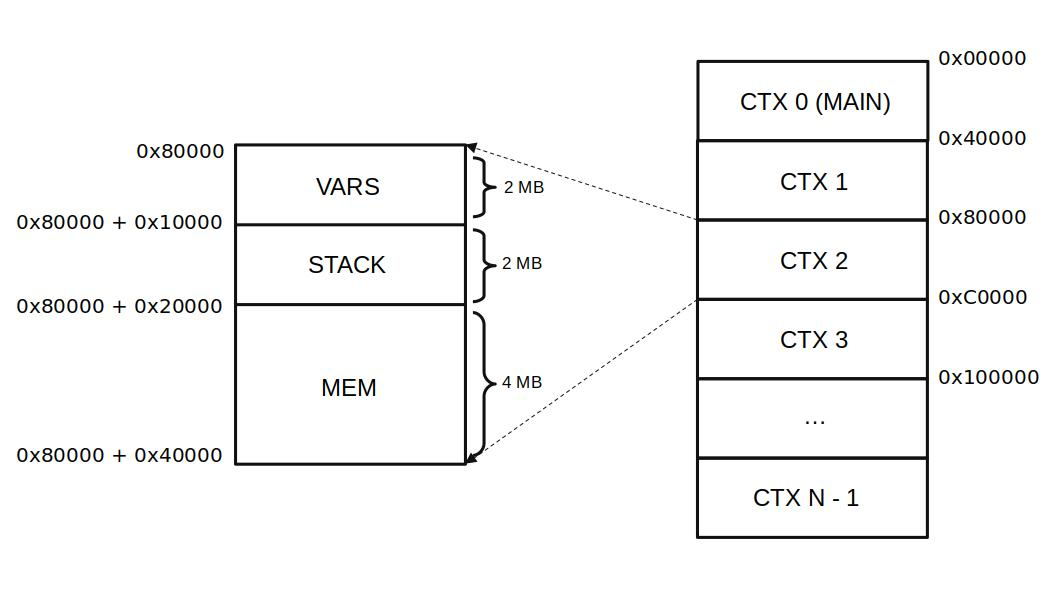
\includegraphics[width=0.6\columnwidth]{\assemblydir/figures/memory-regions}
\caption{Schema of contexts and memory regions of the zkEVM.}
\label{fig:memory-regions}
\end{figure}

In order to allow runtime interaction with memory, zkASM has a couple of instructions to read and write values to it.


\subsubsection{\MLOAD}


\MLOAD is the zkASM instruction used to read a value from a specific address in memory. It takes the pointer address of the memory slot to be read as a parameter. We can store the value that is read in a register of our choosing by using the free input (\texttt{\$}) assignment. 

Suppose that we want to read the memory value stored in the address \texttt{someAddr} in a certain context. The address \texttt{someAddr} is defined by the global variable:
\begin{zkasm}
VAR GLOBAL someAddr
\end{zkasm}

The following zkASM code stores the corresponding value into the register \A:
\begin{zkasm}
$ => A          :MLOAD(someAddr)
\end{zkasm}





\subsubsection{\MSTORE}


\MSTORE is the zkASM instruction used to write a value to a specific address in memory. It takes the pointer address of the memory slot to be read as a parameter, the register that contains the value to be writed must be also specified.

The following example shows how to store in the memory the value of the current context. Note that as the \MSTORE parameter, it is specified the variable that contains the pointer to where current context is stored in the memory. The value stored will be taken from \texttt{CTX} register:
\begin{zkasm}
CTX       :MSTORE(currentCTX)      
\end{zkasm}



\subsubsection{Dealing with the STACK}

A stack machine is a machine in which temporary values for computations are moved to and from a push down stack. Operations over the stack are the typical: \texttt{PUSH}, \texttt{POP}, \texttt{DUP}, \texttt{SWAP}, etc. Since the EVM is a stack-based virtual machine, we reserve an address space to create a stack within the memory of the zkEVM. The classical pointer called \texttt{STACK POINTER} (\texttt{SP}) contains the address of the \textbf{next free position on the} \texttt{STACK}. A \texttt{POP} from the \texttt{STACK} can be implemented as:

\begin{zkasm}
    SP -1 => SP
    $ => A		:MLOAD(SP)
\end{zkasm}

where we decrement \texttt{SP} to reposition it on the last element of the stack and
then we load this element into registry \A. Similarly, a \texttt{PUSH} into the \texttt{STACK} can be implemented as:

\begin{zkasm}
    0		:MSTORE (SP++)
\end{zkasm}

which saves a \texttt{0} at the top of the stack and increments \texttt{SP}. An important note about both the stack and the memory is that the stack pointer and the memory are per context.




\subsubsection{\texttt{MEM\_ALIGN\_RD}}

Although the memory word in zkASM is 256 bits long, in roder to mimic the regular Ethereum Virtual Machine (EVM) memory behavior, zkASM has a specific instructions for accessing memory at the byte level. The instruction \texttt{MEM\_ALIGN\_RD} enables reading 32 bytes starting from an offset of any byte in memory. In this way, two memory registers are read and a the following transformation is applied to virtually obtain a new 32-byte word as a result of the reading.
\begin{align*}
\texttt{val} &= \Bigr[ \texttt{m}_0 \ll 8 \cdot \texttt{offset} \Bigr] \mathbin\Vert \Bigr[ \texttt{m}_1 \gg 256- 8 \cdot \texttt{offset} \Bigr] 
\end{align*}

Here, the symbol $\mathbin\Vert$ denotes string concatenation. The registers must be set as follows before call the \texttt{MEM\_ALIGN\_RD} instruction. We can store the value that is read in a register of our choosing by using the free input (\texttt{\$}) assignment.


\begin{figure}[h!]
\renewcommand{\figurename}{Table}
\[
\begin{array}{|c|c|}
\hline
\mathbf{Register} &\mathtt{MEM\_ALIGN\_RD} \ \mathbf{parameters} \\ \hline
\A & \texttt{Memory Slot of } \mathtt{m_0} \\
\B & \texttt{Memory Slot of } \mathtt{m_1} \\
\C & \texttt{offset} \\
\hline
\end{array}
\]
\caption{\texttt{MEM\_ALIGN\_RD} instruction parameters.}
\label{tab:memory-first-example}
\end{figure}

The following example shows how to read 32 bytes that are stored occupying part of two consecutive zkASM memory words. The read value will be stored in register \A:

\begin{zkasm}
  $ => A          :MLOAD(someAddr)
  $ => B          :MLOAD(someAddr+1)
  16 => C
  ; get memeory value
  $ => A          :MEM_ALIGN_RD
\end{zkasm}

Figure ?? shows how the 32-bytes value will be read for the \texttt{MEM\_ALIGN\_RD} given example.

\begin{figure}[H]
  \centering
  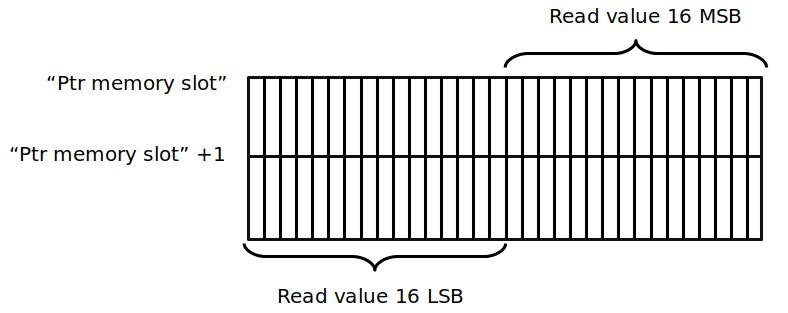
\includegraphics[width=0.8\columnwidth]{\assemblydir/figures/mem-align-wr}
  \caption{Example of how values are read from the memmory using \texttt{MEM\_ALIGN\_RD} with an offset of 16.}
  \label{fig:memory-regions}
\end{figure}

\subsubsection{\texttt{MEM\_ALIGN\_WR}}
\texttt{MEM\_ALIGN\_WR} is equivalent to \texttt{MEM\_ALIGN\_RD} but for writing a 32-byte value. In this case, we have to specify two memory slots that will be written after applying the following transformation to the value to be stored. The registers that contains the value to be stored must also be specified.
\begin{align*}
\texttt{w}_0 &= \Bigr[ \texttt{m}_0 \ \texttt{\&} \ \left(2^{256} - 2^{256-8 \cdot \texttt{offset}} \right) \Bigr] \mathbin\Vert \Bigr[  \texttt{val} \ll 8 \cdot \texttt{offset} \Bigr]  \\
\texttt{w}_1 &= \Bigr[ \texttt{m}_1 \ \texttt{\&} \ \left( \left( 2^{256} - 1\right)  \gg 8 \cdot \texttt{offset}\right) \Bigr] \mathbin\Vert \Bigr[ \texttt{val} \ll 8 \cdot \texttt{offset} \Bigr] 
\end{align*}

\begin{figure}[h!]
\renewcommand{\figurename}{Table}
\[
\begin{array}{|c|c|}
\hline
\mathbf{Register} &\mathtt{MEM\_ALIGN\_WR} \ \mathbf{parameters} \\ \hline
\A & \texttt{Memory Slot of } \mathtt{m_0}  \\
\B & \texttt{Memory Slot of } \mathtt{m_1}  \\
\C & \mathtt{offset} \\
\D & \mathtt{w_0} \\
\E & \mathtt{w_1} \\
\op& \texttt{Value to be written} \\
\hline
\end{array}
\]
\caption{\texttt{MEM\_ALIGN\_WR} instruction parameters.}
\label{tab:memory-first-example}
\end{figure}

The following example shows how to write 32 bytes that are stored occupying part of two consecutive zkASM memory words. The value to be stored will be taken from free input register:

  \begin{zkasm}
  $ => A          :MLOAD(MEM:E)
  $ => B          :MLOAD(MEM:E+1)

  ${memAlignWR_W0(A,mem.bytesToStore,C)} => D                    ; no trust calculate W0
  ${memAlignWR_W1(B,mem.bytesToStore,C)} => E                    ; no trust calculate W1
  $               :MEM_ALIGN_WR,MLOAD(bytesToStore)
\end{zkasm}

\subsubsection{\texttt{MEM\_ALIGN\_WR8}}

\texttt{MEM\_ALIGN\_WR8} allows writing only 8 bits of a specific memory slot. In this case, we have to specify the memory slot to be written, the register that contains the byte to be stored, and the offset value that situates the byte in a specific position of the 32-byte word. The value will be written after applying the following transformation:
\begin{align*}
\texttt{w}_0 &= \Bigr[ \texttt{m}_0 \ \texttt{\&} \ \left( \texttt{maskByte} \gg 8 \cdot \texttt{offset} \right) \Bigr]  \mathbin\Vert \Bigr[ \left( \texttt{bits} \ \texttt{\&} \ \texttt{0xFF} \right)  \ll 8 \cdot \left( 31-\texttt{offset}\right) \Bigr] 
\end{align*}
where $\texttt{maskByte}$ equals $2^{256} - 1$. 

\begin{figure}[h!]
\renewcommand{\figurename}{Table}
\[
\begin{array}{|c|c|}
\hline
\mathbf{Register} &\mathtt{MEM\_ALIGN\_WR8} \ \textbf{parameters} \\ \hline
\A & \texttt{Memory Slot of } \mathtt{m_0} \\
\C & \mathtt{offset} \\
\D & \mathtt{w_0} \\
\op& \texttt{Value to be written} \\
\hline
\end{array}
\]
\caption{\texttt{MEM\_ALIGN\_WR8} instruction parameters.}
\label{tab:memory-first-example}
\end{figure}

The following example shows how to write $1$ bytes stored in the byte $4$ of a specific storage slot. The value to be stored will be taken from \B register:

\begin{zkasm}
4 => C
$ => A          :MLOAD(someAddr)
${memAlignWR8_W0(A,B,C)} => D  ; no trust calculate W0
B               :MEM_ALIGN_WR8 ; only use LSB of B, rest of bytes could be non zero
\end{zkasm}

\subsection{Storage Related Instructions}

Polygon zkEVM, like Ethereum L1, has a storage component for storing persistent on-chain data, which includes the balances of all accounts, their nonces, and the state of all deployed smart contracts along with their codes. The data that forms the state is represented as cryptographic trie, but while Ethereum L1 uses a modified Patricia tree with Keccak256 as the hash operation, Polygon zkEVM uses a binary sparse Merkle tree with Poseidon as the hash operation (refer to the technical documents regarding the zkEVM bridge annex A to learn more about sparse Merkle trees).

Poseidon is a hash function that's specifically designed for use in zero-knowledge applications, as it's meant to operate with values of a prime field and it has been proven to be much more performant than Keccak256 in zero-knowledge constructions like those used in Polygon zkEVM. Moreover Poseidon hash has an input named capacity, which can be used as an extra input value.

Barely, the Polygon zkEVM state tree is a key-value structure in which the integrity can be ensured by a 256-bit value known as the state root. Each entry in the tree is a leaf and directly stores a 256-bit value. Additionally, the index position of that leaf in the tree corresponds to the 256-bits of the key. As can be seen in Figure X, since the keys are 256-bits in length, the tree has 32 levels and a total capacity of $2^{256}$ leaves.


\begin{figure}[H]
\centering
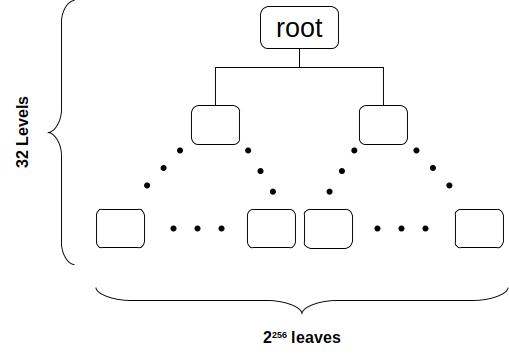
\includegraphics[width=0.6\columnwidth]{\assemblydir/figures/state-trie}
\caption{Polygon zkEVM state trie.}
\label{fig:hashk-add-bytes}
\end{figure}

Since five different types of values can be stored, a distinction must be made among the five types of leaves. Table X shows the relation between leaf type and the corresponding data types that they contain.

\begin{figure}[h!]
\renewcommand{\figurename}{Table}
\[
\begin{array}{|c|c|}
\hline
\mathbf{Leaf~type} &\mathbf{Data~type} \\ \hline
\mathtt{0} & \mathtt{Account~balance} \\
\mathtt{1} & \mathtt{Account~nonce} \\
\mathtt{2} & \mathtt{Contract~code~hash} \\
\mathtt{3} & \mathtt{Contract~storage~slot~value} \\
\mathtt{4} & \mathtt{Contract~code~length} \\
\hline
\end{array}
\]
\caption{Polygon zkEVM state tree leaf types.}
\label{tab:memory-first-example}
\end{figure}


For each leaf entered in the tree its key is computed as follows:

$$\texttt{key} = \texttt{Poseidon}(\texttt{key\_seed})$$

where \texttt{key\_seed} is a $32$-bytes integer constructed as follows:
\[
\texttt{key\_seed} = (\texttt{account\_address} \mid\mid \texttt{0x00000000} \mid\mid \texttt{leaf\_type} \mid\mid \texttt{0x00000000})
\]
being $\texttt{account\_address} \in \{0, 1, \dots, 2^{160} - 1\}$ is a $20$-bytes integer and $\texttt{leaf\_type} \in \{0, 1, \dots, 2^{32} - 1\}$ a $4$-bytes integer.

The capacity of the Poseidon's instance used when computing keys is always zero except in the case where the leaf corresponds to a contract storage slot value (leaf type 3), in which case the capacity is directly set to the storage slot pointer. It's important to note that because the contract storage slot pointer is not encoded in the 32-byte input, if we do not use the capacity, all storage slots for the same contract would lead to the same state tree leaf.

Te value sored in the leaf has the following structure:
\[
(v_0, \dots, v_7)
\]
codifying a $256$-bits unsigned integer, where $v_i \in \FF_p$ are bounded to $32$-bits each. 

In order to allow runtime interaction with the Polygon zkEVM state tree zkASM has a couple of instructions to read and write values on it.

\subsubsection{\texttt{SLOAD}}

\texttt{SLOAD} is the zkASM instruction used to read a value from a leaf in the state tree. It takes Poseidon's ``Input" and ``Capacity" parameters, along with the leaf type, to compute the key of the leaf to be read. The registers must be set as follows before call the \texttt{SLOAD} instruction.

\begin{figure}[h!]
\renewcommand{\figurename}{Table}
\[
\begin{array}{|c|c|}
\hline
\mathbf{Register} &\texttt{SLOAD } \textbf{parameters} \\ \hline
\A & \mathtt{Account~address} \\
\B & \mathtt{Leaf~type} \\
\C & \mathtt{Contract~storage~slot~pointer~(capacity)} \\
\hline
\end{array}
\]
\caption{\texttt{SLOAD} instruction parameters.}
\label{tab:memory-first-example}
\end{figure}

We can store the value that is read in a register of our choosing by using the free input (\texttt{\$}) assignment.

The following example shows how to read the balance of a specific account, the value that is read will be stored in the \E register:

\begin{zkasm}
  someAccountAddr => A          
  0 => B      
  0 => C          
  $ => E          :SLOAD
\end{zkasm}

The following example shows how to read a storage slot of a specific contract, the value that is read will be stored in the \E register:

\begin{zkasm}
  someAccountAddr => A          
  3 => B      
  storageSlotPtr => C 
  $ => E          :SLOAD
\end{zkasm}

\subsubsection{\texttt{SSTORE}}

\texttt{SSTORE} is the zkASM instruction used to store a value to a leaf in the state tree. It takes Poseidon's ``Input" and ``Capacity" parameters, along with the leaf type, to compute the key of the leaf to be writen, in addition takes the value to be written. The registers must be set as follows before call the \texttt{SSTORE} instruction.

\begin{figure}[h!]
  \renewcommand{\figurename}{Table}
  \[
  \begin{array}{|c|c|}
  \hline
  \mathbf{Register} &\texttt{SSTORE } \textbf{parameters} \\ \hline
  \A & \mathtt{Account~address} \\
  \B & \mathtt{Leaf~type} \\
  \C & \mathtt{Contract~storage~slot~pointer~(capacity)} \\
  \D & \mathtt{Value~to~write} \\
  \hline
  \end{array}
  \]
  \caption{\texttt{SSTORE} instruction parameters.}
  \label{tab:memory-first-example}
  \end{figure}
  
  The following example shows how to write a storage slot of a specific contract:

  \begin{zkasm}
    someAccountAddr => A          
    3 => B      
    storageSlotPtr => C          
    value => D         
    A               :SSTORE
  \end{zkasm}




%%%%%%%%%%%%%%%%%%%%%%%%%%%%%%%%%%%%%%%%%%%%%%%%%%%%%%%%%%%%%%%

\subsection{Binary-Related Instructions}

The arithmetic operators are used to perform arithmetic mathematical operations on numeric data stored in registers.

\subsubsection{\ADD}

\ADD is used to sum the content of the registers \A and \B, the result will be treated as a free input. The following example shows how to use \ADD instruction.

\begin{zkasm}
    val1 => A          
    val2 => B          
    
    $ => C             :ADD ; [ val1 + val2 => C]
\end{zkasm}

\subsubsection{\SUB}

\SUB is used to subtract de content fo register \B to \A, the result will be treated as a free input. The following example shows how to use \SUB instruction.

\begin{zkasm}
    val1 => A          
    val2 => B          
    
    $ => C             :SUB ; [ val1 - val2 => C]
\end{zkasm}



\subsubsection{\LT}

\LT instruction is used to compare the values of the registers \A and \B as \textbf{unsigned integers}. The output of the operation will be $1$ if \A is actually lower than \B (that is, $\A < \B$) and $0$ otherwise (that is, $\A \geq \B$). The output of the instruction will be treated as a free input. The next lines of code show an example on how to use \LT instruction:

\begin{zkasm}
valA => A
valB => B

$ => C			:LT ; [1 if A < B, 0 if A <= B]
\end{zkasm}





\subsubsection{\SLT}

\SLT instruction is used to compare the values of the registers \A and \B as \textbf{signed integers}, explained in Section \ref{sec:binary-sm}. The output of the operation will be $1$ if \A is actually lower than \B (that is, $\A < \B$) and $0$ otherwise (that is, $\A \geq \B$). The output of the instruction will be treated as a free input. The next lines of code show an example on how to use \SLT instruction:

\begin{zkasm}
    valA => A
    valB => B
    
    $ => C			:SLT ; [1 if A < B, 0 if A <= B]
\end{zkasm}


\subsubsection{\EQ}

\EQ instruction is used to compare the equality relationship between the values of the registers \A and \B. The output of the operation will be $1$ if \A is equal to \B (that is, $\A = \B$) and $0$ otherwise (that is, $\A \neq \B$). The output of the instruction will be treated as a free input. The next lines of code show an example on how to use \EQ instruction:

\begin{zkasm}
    valA => A
    valB => B
    
    $ => C			:EQ ; [1 if A = B, 0 if A != B]
\end{zkasm}


\subsubsection{\AND}


\AND instruction is used to perform the bit-wise \AND operation between registers \A and \B, as explained in Section \ref{sec:binary-sm}. The output of the instruction will be treated as a free input. The next lines of code show an example on how to use \AND instruction:

\begin{zkasm}
    valA => A
    valB => B
    
    $ => C			:AND
\end{zkasm}

For sake of completeness, let us propose a more concrete example, where we assign the value $\texttt{0xDBn}$ to \A and the value $\texttt{0x86n}$ to \B. The result of the bit-wise \AND operation is going to be \texttt{0x82n} because
\[
\A = \texttt{0b11011011}, \quad \B = \texttt{0b10000110} \Longrightarrow \C = \texttt{0b10000010}.
\]

\begin{zkasm}
    0xDBn => A
    0x86n => B
    
    $ => C			:AND ; C = 0x82n
\end{zkasm}

\subsubsection{\OR}

\OR instruction is used to perform the bit-wise \OR operation between registers \A and \B, as explained in Section \ref{sec:binary-sm}. The output of the instruction will be treated as a free input. The next lines of code show an example on how to use \OR instruction:

\begin{zkasm}
    valA => A
    valB => B
    
    $ => C			:OR
\end{zkasm}

For sake of completeness, let us propose a more concrete example, where we assign the value $\texttt{0xDBn}$ to \A and the value $\texttt{0x86n}$ to \B. The result of the bit-wise \OR operation is going to be \texttt{0xDFn} because
\[
\A = \texttt{0b11011011}, \quad \B = \texttt{0b10000110} \Longrightarrow \C = \texttt{0b11011111}.
\]

\begin{zkasm}
    0xDBn => A
    0x86n => B
    
    $ => C			:OR ; C = 0xDFn
\end{zkasm}



\subsubsection{\XOR}

\XOR instruction is used to perform the bit-wise \XOR operation between registers \A and \B, as explained in Section \ref{sec:binary-sm}. The output of the instruction will be treated as a free input. The next lines of code show an example on how to use \XOR instruction:

\begin{zkasm}
    valA => A
    valB => B
    
    $ => C			:XOR
\end{zkasm}

For sake of completeness, let us propose a more concrete example, where we assign the value $\texttt{0xDBn}$ to \A and the value $\texttt{0x86n}$ to \B. The result of the bit-wise \XOR operation is going to be \texttt{0x5Dn} because
\[
\A = \texttt{0b11011011}, \quad \B = \texttt{0b10000110} \Longrightarrow \C = \texttt{0b01011101}.
\]

\begin{zkasm}
    0xDBn => A
    0x86n => B
    
    $ => C			:XOR ; C = 0x5Dn
\end{zkasm}





%%%%%%%%%%%%%%%%%%%%%%%%%%%%%%%%%%%%%%%%%%%%%%%%%%%%%%%%%%%%%%%
\subsection{Arithmetic-Related Instructions}

\subsubsection{\ARITH}

The \ARITH instruction allows to check field operations. More specifically, it checks a combination of an addition and a product, as explained in Section \ref{sec:arith-sm}. Before calling the \ARITH instruction, registers \A, \B, and \C must be set. The equation that follows will be evaluated using the values of these $3$ registers. It is necessary to specify where the result of the evaluation will be stored. If the evaluation results in an overflow of the output register, the overflow value will be stored in register \D. More specifically, the equation that checks the \ARITH instruction is the following one:

\[
\D \cdot 2^{256} + \op = \A \cdot \B + \C
\]

The following example shows how to use \ARITH instruction. The result of the evaluation will be stored in register \A, and if there is an overflow, it will be stored in register \D:
\begin{zkasm}
    valA => A          
    valB => B          
    valC => C
    A            :ARITH ; [ valA * valB + valC => [D,A]]
\end{zkasm}





\subsubsection{\ARITHADDDIFF}

The \ARITHADDDIFF instruction allows to perform additions $P + Q$ over the elliptic curve defined in Section \ref{sec:arith-sm}. This instruction can not perform doublings, since the input points to be added are supposed to be different. This is not explicitly check, but since the doubling formula differs a lot from the distinct point addition formula, the result will be wrong if $P = Q$. The input parameters of the instruction are specified in the table below:

\begin{figure}[h!]
\renewcommand{\figurename}{Table}
\[
\begin{array}{|c|c|}
\hline
\mathbf{Register} &\texttt{ARITH\_ECADD\_DIFFERENT } \textbf{parameters} \\ \hline
\A & x_1, \mathtt{~x~coordinate~of~}P \\
\B & y_1, \mathtt{~y~coordinate~of~}P \\
\C & x_2, \mathtt{~x~coordinate~of~}Q \\
\D & y_2, \mathtt{~y~coordinate~of~}Q \\
\E & x_3, \mathtt{~x~coordinate~of~}P+Q \\
\op & y_3, \mathtt{~y~coordinate~of~}P+Q \\
\hline
\end{array}
\]
\caption{\ARITHADDDIFF instruction parameters.}
\label{tab:memory-first-example}
\end{figure}

An example on how to use the \ARITHADDDIFF instruction can be seen in the code blow. Observe that we make use of the executor implemented functions \texttt{xAddPointEc(A,B,C,D)} and \texttt{yAddPointEc(A,B,C,D)} which compute the $x$ and the $y$ coordinate of $P + Q$ being $P = (A, B)$ and $Q = (C, D)$ whenever $P \neq Q$. After this is computed, the $x$ coordinate of $P + Q$ is is stored into the memory slot given by the address \texttt{addX} and, similarly, the $y$ coordinate of $P + Q$ is pushed into the memory slot given by the address \texttt{addY}. If we have used incorrect values for the coordinates of $P + Q$, an executor error will pop. This will also be captured when the proof of the batch is generated, since the instruction invocation fills the polynomials of the Arithmetic State Machine correctly. 

\begin{zkasm}
$ => A  						:MLOAD(Px)
$ => B  						:MLOAD(Py)
$ => C  						:MLOAD(Qx)
$ => D  						:MLOAD(Qy)
${xAddPointEc(A,B,C,D)} => E  	:MSTORE(addX)
${yAddPointEc(A,B,C,D)} 		:ARITH_ECADD_DIFFERENT, MSTORE(addY)
\end{zkasm}


\subsubsection{\ARITHADDSAME}

The \ARITHADDSAME instruction allows to perform point doublings $2P$ over the elliptic curve defined in Section \ref{sec:arith-sm}. The input parameters of the instruction are specified in the table below:

\begin{figure}[h!]
\renewcommand{\figurename}{Table}
\[
\begin{array}{|c|c|}
\hline
\mathbf{Register} &\texttt{ARITH\_ECADD\_DIFFERENT } \textbf{parameters} \\ \hline
\A & x_1, \mathtt{~x~coordinate~of~}P \\
\B & y_1, \mathtt{~y~coordinate~of~}P \\
\E & x_3, \mathtt{~x~coordinate~of~}2P \\
\op & y_3, \mathtt{~y~coordinate~of~}2P \\
\hline
\end{array}
\]
\caption{\ARITHADDDIFF instruction parameters.}
\label{tab:memory-first-example}
\end{figure}

An example on how to use the \ARITHADDSAME instruction can be seen in the code blow. Observe that we make use of the executor implemented functions \texttt{xDblPointEc(A,B)} and \texttt{yDblPointEc(A,B)} which compute the $x$ and the $y$ coordinate of $2P$ being $P = (A, B)$. After this is computed, the $x$ coordinate of $2P$ is is stored into the memory slot given by the address \texttt{doublePx} and, similarly, the $y$ coordinate of $2P$ is pushed into the memory slot given by the address \texttt{doublePy}. If we have used incorrect values for the coordinates of $2P$, an executor error will pop. This will also be captured when the proof of the batch is generated, since the instruction invocation fills the polynomials of the Arithmetic State Machine correctly. 

\begin{zkasm}
$ => A  					:MLOAD(Px)
$ => B  					:MLOAD(Py)

${xDblPointEc(A,B)} => E  	:MSTORE(doublePx)
${yDblPointEc(A,B)} 		:ARITH_ECADD_SAME, MSTORE(doublePy)
\end{zkasm}









%%%%%%%%%%%%%%%%%%%%%%%%%%%%%%%%%%%%%%%%%%%%%%%%%%%%%%%%%%%%%%%
\subsection{Execution Control Flow Related Instructions}

In order to allow to conditional branch execution of the zkASM programs, 4 different instruction has been included in zkASM instructios set.

\subsubsection{\JMP} % Jump
\JMP is an unconditional jump instruction that always causes a jump in the program's execution flow, regardless of any conditions. It takes an address of the ROM as a parameter to continue the execution flow. To avoid using numeric pointers for jumps, zkASM allows jump destinations to be aliased with custom names. The compiler resolves these aliases and substitutes them with pointers later on.

The following code shows the general usage of \JMP instruction:

\begin{zkasm}

; ...
; Executed Code
; ...

                :JMP(destinationLabel)

; ... 
; Non Executed Code
; ... 

destinationLabel:

; ...
; Executed Code
; ...

\end{zkasm}


\subsubsection{\JMPN} % Jump if Negative

\JMPN is a conditional jump instruction that causes a jump in the program's execution flow if a specified register contains a negative number. It takes the address of the ROM as a parameter to continue the execution flow. The register that contains the value to be evaluated must also be specified.

In the following example, the execution flow will be redirected to \texttt{stackUnderflow} in the case that the evaluation of $\SP - 2$ leads to a negative number.

\begin{zkasm}
; check stack underflow
SP - 2          :JMPN(stackUnderflow)
\end{zkasm}





\subsubsection{\JMPC} % Conditional jump, if a condition is fullfiled

\JMPC is a condititional jump instruction that causes a jump in the program's execution flow if a specified condition is evaluated  as true. It is used along with the following comparative instructions.
\begin{itemize}
\item \EQ: Evaluates if register \A value is equal to register \B value.
\item \LT: Evaluates if register \A value is less than register \B value.
\item \SLT: Evaluates if register \A value is less than register \B value also comparing negative values.
\end{itemize}

In the following example, the execution flow will be redirected to \texttt{absIsNeg} in the case that the value contained in register \A (namely \val) is a negative number.

\begin{zkasm}
val => A
0 => B
$          :SLT, JMPC(absIsNeg)
\end{zkasm}





\subsubsection{\texttt{JPMZ}} % Jump if Zero

\texttt{JPMZ} is a conditional jump instruction that causes a jump in the program's exectuion flow if a specified register contains a 0. In the following example, the execution flow will be redirected to \texttt{readCode} in the case that the value contained in register \A (namely \val) is $0$.

\begin{zkasm}
val => A
A                   :JMPZ(readCode)
\end{zkasm}

\subsubsection{\ASSERT}
\ASSERT is used to ensure that a given register has the same value as register \A. A failing assertion, meaning that the values are unequal, will stop execution and throw error during runtime. Additionally, an execution that contains a failing assertion cannot generate a valid CI proof.

The following code will compare $\val_1$ with $\val_2$, and if they are not equal the execution will be immediately stopped:

\begin{zkasm}
val1 => A
val2 => B
B    :ASSERT
\end{zkasm}





\subsubsection{Subroutines (\CALL and \RETURN)}


Subroutines allow breaking down the code into smaller sections that can be called by using only a \CALL instruction. A subroutine is designed to be reusable and can be called by other parts of the program. The code of a subroutine always ends with a \RETURN instruction. When a subroutine is called, control is transferred from the main program to the subroutine. The subroutine then executes its code and, when it's finished, control is returned to the point in the main program immediately following the point where the subroutine was called.

An example of subroutine can be the \texttt{ecrecover\_tx} subrutine used in the zkEVM ROM, it is used to recover the signer of a specific ethereum transaction. zkASM code of \texttt{ecrecover\_tx } subrutine can be found \href[]{https://github.com/0xPolygonHermez/zkevm-rom/blob/b27579b89a95a344d09656490a50df5fc67c8417/main/ecrecover/ecrecover.zkasm}{here}.

The following zkASM code shows how to use the \texttt{ecrecover\_tx} subroutine. Once the subroutine is executed, the code will continue on the following line and the recovered address will be in register \A:
\begin{zkasm}
0xd9eba16ed0ecae432b71fe008c98cc872bb4cc214d3220a36f365326cf807d68n => A ; Tx hash
0xddd0a7290af9526056b4e35a077b9a11b513aa0028ec6c9880948544508f3c63n => B ; r
0x265e99e47ad31bb2cab9646c504576b3abc6939a1710afc08cbf3034d73214b8n => C ; s
0x1cn => D ; v
                                        :CALL(ecrecover_tx)
\end{zkasm}





\subsubsection{\REPEAT}

Although jumps are enough in order to build program loops, a \REPEAT instruction has been introduced in order to easily repeat a certain line of code. The \REPEAT instruction makes use of the \RCX register in order to parametrize the number of times the code should be repeated. To illustrate how to use the \REPEAT instruction, we are going to propose an example:

\begin{zkasm}
10 => A
14 => RCX
A + 2 => A  :REPEAT(RCX)

40  :ASSERT 
\end{zkasm}

The previous code assigns $10$ to the \A register and $14$ to the repeat counter \RCX. After that, invokes an addition by two units of the \A register, together with the \REPEAT instruction with parameter \RCX. This will make the line of code 

\begin{zkasm}
A + 2 => A
\end{zkasm}

to repeat a total amount of $15$ times, the first one written explicitly in the code and the other $14$ times produced by the \REPEAT instruction. This is something the user should take into account. After that, the \A register will contain the value
\[
10 + 15 \cdot 2 = 40.
\]
Hence, an \ASSERT can be invoked against the value $40$, since \A should be $\op = 40$.  




%%%%%%%%%%%%%%%%%%%%%%%%%%%%%%%%%%%%%%%%%%%%%%%%%%%%%%%%%%%%%%%
\subsection{Hash Related Instructions}

Both implementations in the zkEVM of each of the hashes is exactly the same, henceforth what we explain in this section for the \texttt{KECCAK-256} hash can be applied also for the \texttt{Poseidon} hash. There are $4$ instructions referent to \texttt{KECCAK-256} hashes in the zkEVM assembly language: \HASHK, \HASHKONE, \HASHKLEN and \HASHKDIGEST. Each of them has a different purpose:

\begin{itemize}

\item \HASHK: This instruction is in charge of consecutively keep introducing bytes into the input of the hash. Via this instruction we can introduce a maximum amount of $32$ bytes at the same time. 

\item \HASHKONE: This instruction is does actually the same that the previous instruction but only can introduce $1$ byte at the time. 

\item \HASHKLEN: This instruction is the one that actually performs the hash but actually do not retrieve its digest. 

\item \HASHKDIGEST: This instruction retrieves the previous hash digest performed using the \HASHKLEN instruction. 

\end{itemize}

Similarly, there are $4$ instructions referent to \texttt{Poseidon} hashes in the zkEVM assembly language: \HASHP, \HASHPONE, \HASHPLEN and \HASHPDIGEST. Each of them mirrors the same instruction explained in the \texttt{KECCAK-256} case. 



\subsubsection{\HASHK}

Since hash functions can hash an arbitrarily large amount of data but our registers are limited to $32$ bytes, we need a procedure to sequentially keep introducing bytes in order to be hashed together. This is what this instruction is providing: it allows to append from $1$ to $32$ bytes to the current input of the hash. The following registers will be relevant in this instruction: $\mathtt{D_0}$ and \texttt{HASHPOS}. The former will contain the desired bytes we want to append and the later will contain the index of the next position of the bytes array of the input of the hash that we will start to fill. That is, this register will contain the total input bytes that we have previously introduced up to this precise moment. 

\begin{figure}[H]
\centering
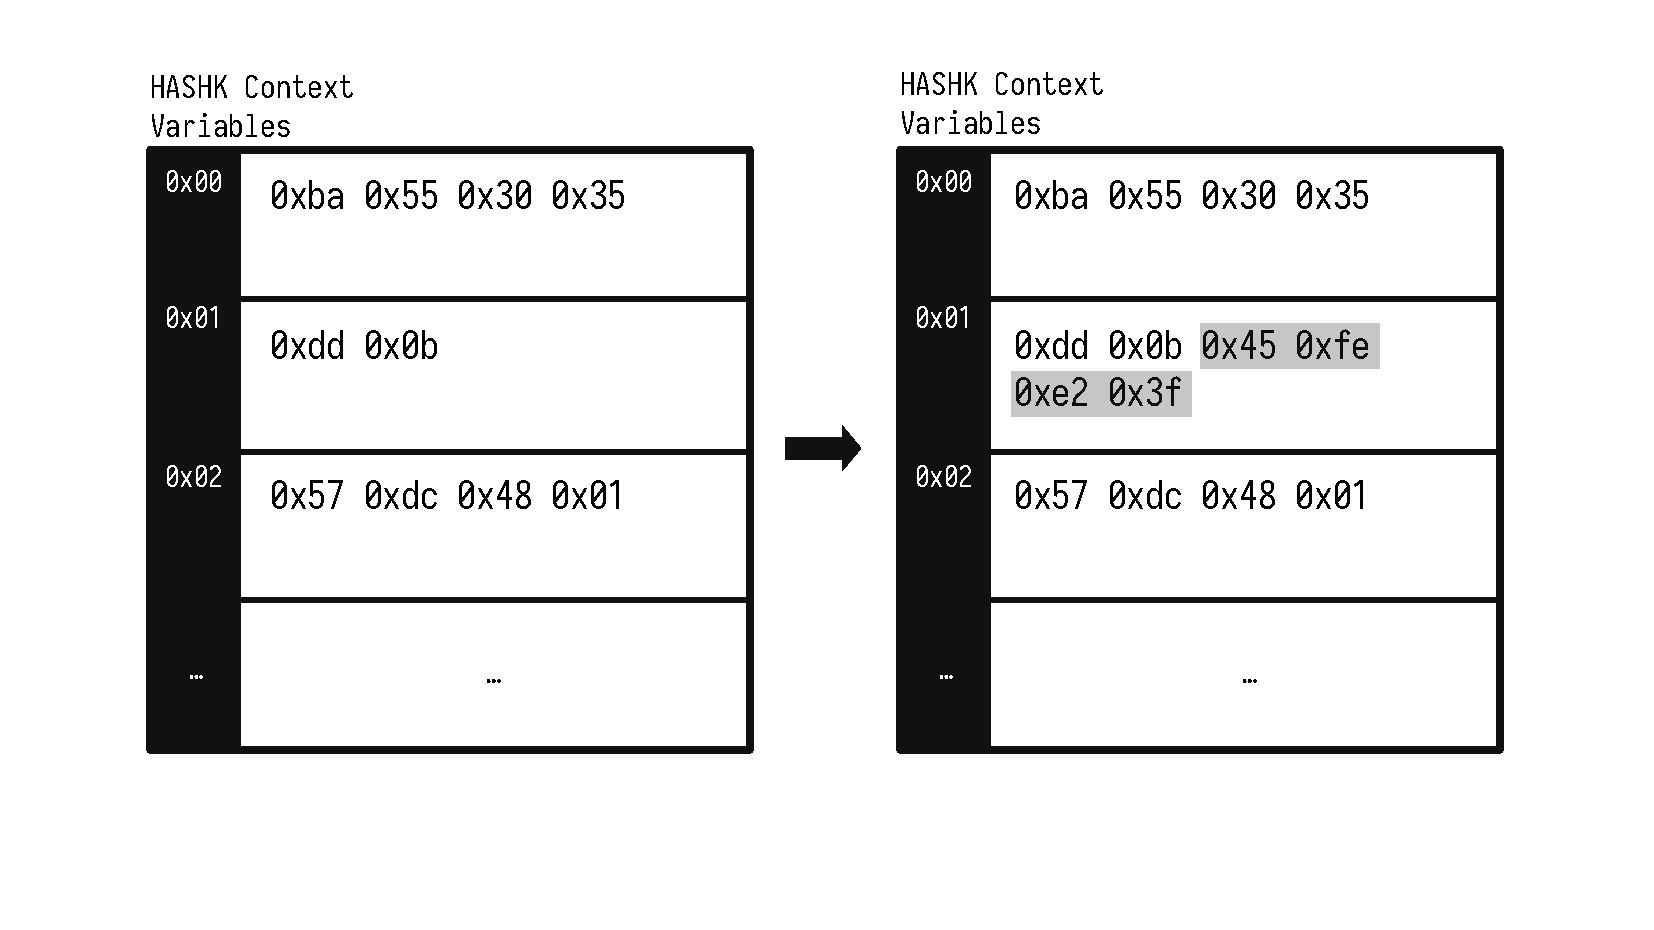
\includegraphics[width=0.6\columnwidth]{\assemblydir/figures/hashk-add-bytes}
\caption{Schema of the \HASHK instruction.}
\label{fig:hashk-add-bytes}
\end{figure}

The typical use of the \HASHK instruction in the zkASM language is the following one:

\begin{zkasm}
op	:HASHK(addr)
\end{zkasm}

The \op placeholder will usually be a register or a register operation like the following one: 

\begin{zkasm}
A + 1	:HASHK(addr)
\end{zkasm}

We can perform several hashes at the same time, each of them being stored in its corresponding address. Then, we can keep filling each of the addresses' bytes without perturbing the other ones. We can specify the address using the register \E, which is the one used to store addresses $256$-bits, or using a hard coded number. The value $0$ is usually used as an address, which is reserved for storing specific hashes. %TODO: what hashes?

\begin{zkasm}
A + 1	:HASHK(E)
\end{zkasm}

The former instruction will append the bytes of the current value of \A + 1 into the input of the hash function we want to perform within the bytes attached to the address \E. 

To formalise what the \HASHK instruction does, let $(\op_0, \op_1, \dots, \op_{31})$ be the byte decomposition of the \op variable. We will denote $\mathtt{trunc_{D_0}}(\op)$ by the byte decomposition of \op truncated at the $\mathtt{D_0}$ position. More precisely, 
\[
\mathtt{trunc_{D_0}(\op)} = (\op_0, \op_1, \dots, \op_{\D_0-1}).
\]

Let $\mathtt{hashk}[\texttt{addr}] = (h_0, \dots, h_{\texttt{HASHPOS}})$ be the current array of bytes that we are willing to hash at a certain address \texttt{addr}. The \HASHK instruction will append the $\mathtt{trunc_{D_0}}(\op)$ array into the $\mathtt{hashk}$ one, so that the next state of the (temporal) input of the hash will become 
\[
\mathtt{hashk}[\texttt{addr}] \nextStep = (h_0, \dots, h_{\texttt{HASHPOS}}, \op_0, \op_1, \dots, \op_{\D_0-1})
\]

At the end of this operation, we increase the value of the \texttt{HASHPOS} register in $\mathtt{D_0}$:
\[
\mathtt{HASHPOS} \nextStep = \mathtt{HASHPOS} + \mathtt{D_0}.
\]

Let us propose the following simple example: suppose that we want to hash a single byte concatenated with the first $31$ bytes of a $32$-bytes integer, each of them contained in the registers $\A$ and $\B$ respectively. To that we will use the address \texttt{0x03} stored in the register \E. First of all, we should ensure that our current hash position is $0$, because we are actually starting a new hash.

\begin{zkasm}
0x03 => E
0 => HASHPOS
\end{zkasm}

At this moment
\[
\texttt{hashk}[\texttt{0x03}] = \emptyset.
\]

Later on, we will start adding the single byte of \A into the hash input. Observe that we should assign the length $1$ into the register \D because we need to specify the length value in bytes when using the \HASHK instruction. 

\begin{zkasm}
1 => D
A				:HASHK(E)
\end{zkasm}

Now, we update the array
\[
\texttt{hashk}[\texttt{0x03}] = (a)
\]
where $a$ denotes the current value of the register \A. Moreover, \texttt{HASHPOS} increased in $1$:
\[
\texttt{HASHPOS} \nextStep = \texttt{HASHPOS} + 1.
\]

Now, we do the same with the register \B

\begin{zkasm}
31 => D
B				:HASHK(E)
\end{zkasm}

Finally, the corresponding hash array is the following
\[
\texttt{hashk}[\texttt{0x03}] = (a, b_0, b_1, \dots, b_{30})
\]
where $(b_0, \dots, b_{30}) = \mathtt{trunc}_{31}(\B)$ are the first $31$ bytes of the register \B, which is actually the string we want to hash. Moreover, \texttt{HASHPOS} increased in $31$:
\[
\texttt{HASHPOS} \nextStep = \texttt{HASHPOS} + 31.
\]


\subsubsection{\HASHKONE}

The instruction \HASHKONE performs in the same way that \HASHK but the register $\D_0$ is not relevant here, because the size of the input string is always of $1$ byte. 


\subsubsection{\HASHKLEN}

As commented before, this instruction is actually the one that computes the hash digest and stores it internally, to later on be acquired via the \HASHKDIGEST instruction. This instruction also uses the first $32$ bytes of the \op intermediate value in order to specify the length within all the bytes stored in the specified address that will be hashed. Therefore, the total amount of bytes we can hash is $2^{32}$. 

\begin{figure}[H]
\centering
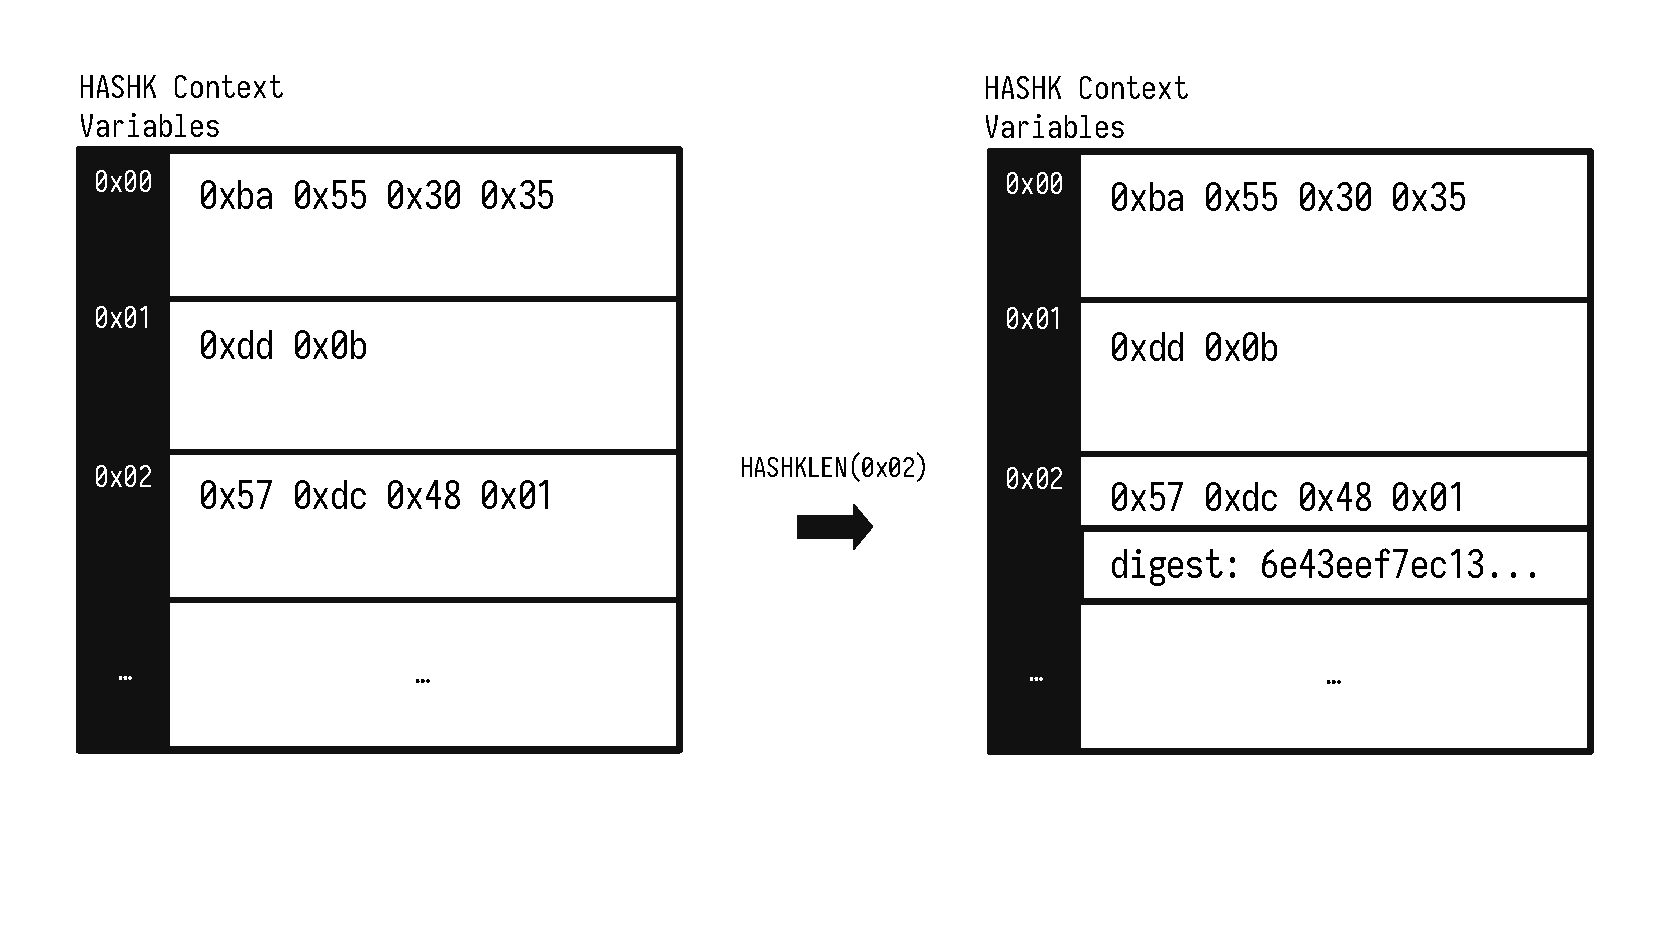
\includegraphics[width=0.6\columnwidth]{\assemblydir/figures/hashklen}
\caption{Schema of the \HASHKLEN instruction.}
\label{fig:hashklen}
\end{figure}


Following the previous example, the line of zkASM that we need to execute in this step is the following one:

\begin{zkasm}
HASHPOS	:HASHKLEN(E)
\end{zkasm}

Recall that \texttt{HASHPOS} value at the current state is $32$ because we want to hash a total amount of $32$ bytes. 


More specifically, if $(h_1, \dots, h_k)$ is the input array attached to a specific address $\texttt{addr}$ (that is, $\mathtt{hashk}[\texttt{addr}] = (h_1, \dots, h_k)$ with the previous notation), the instruction

\begin{zkasm}
len		:HASHKLEN(addr)
\end{zkasm}

internally stores the digest
\[
d = \texttt{KECCAK-256}(h_1, \dots, h_k).
\]

Observe that we should have that $k = \texttt{len}$. Otherwise, the \HASHKLEN instruction will get an error. % TODO: This checks are checking the integrity of the memory?




\subsubsection{\HASHKDIGEST}

This usual way we are invoking this instruction is the following 

\begin{zkasm}
$ => REG	:HASHKDIGEST(E)
\end{zkasm}

Meaning that we are storing the digest of the hash attached to the address $\E$ into the register \texttt{REG}. The hash digest is introduced as a free input using the \texttt{\$ =>} operator. In our example, if we want to assign the digest of the hash to the register \D, we would use the following line

\begin{zkasm}
$ => D		:HASHKDIGEST(E)
\end{zkasm}


%TODO: Counters needs to be incremented.



